\documentclass[a4paper]{article}
%\usepackage{vntex}
%\usepackage[english,vietnam]{babel}
\usepackage[english]{babel}
%\usepackage[utf8]{inputenc}

%\usepackage[utf8]{inputenc}
%\usepackage[francais]{babel}
\usepackage{a4wide,amssymb,epsfig,latexsym,array,hhline,fancyhdr}

\usepackage{amsmath}
\usepackage{amsthm}
\usepackage{multicol,longtable,amscd}
\usepackage{diagbox}%Make diagonal lines in tables
\usepackage{booktabs}
\usepackage{alltt}
\usepackage[framemethod=tikz]{mdframed}% For highlighting paragraph backgrounds
\usepackage{caption,subcaption}
\usepackage{xcolor}
\usepackage{lastpage}
\usepackage[lined,boxed,commentsnumbered]{algorithm2e}
\usepackage{enumerate}
\usepackage{color}
\usepackage{graphicx}							% Standard graphics package
\usepackage{array}
\usepackage{tabularx, caption}
\usepackage{multirow}
\usepackage{multicol}
\usepackage{rotating}
\usepackage{graphics}
\usepackage{geometry}
\usepackage{setspace}
\usepackage{epsfig}
\usepackage{tikz}
\usetikzlibrary{arrows,snakes,backgrounds}
\usepackage[unicode]{hyperref}
\hypersetup{urlcolor=blue,linkcolor=black,citecolor=black,colorlinks=true}
\urlstyle{same}
%\usepackage{pstcol} 							% PSTricks with the standard color package
\usepackage[export]{adjustbox}
%%%%%%%%%%%%%%%%%%%%code format
\usepackage{listings}
\usepackage[breakable]{tcolorbox}
\usepackage{parskip} % Stop auto-indenting (to mimic markdown behaviour)

\usepackage{iftex}
\ifPDFTeX
	\usepackage[T1]{fontenc}
	\usepackage{mathpazo}
\else
	\usepackage{fontspec}
\fi

% Basic figure setup, for now with no caption control since it's done
% automatically by Pandoc (which extracts ![](path) syntax from Markdown).
\usepackage{graphicx}
% Maintain compatibility with old templates. Remove in nbconvert 6.0
\let\Oldincludegraphics\includegraphics
% Ensure that by default, figures have no caption (until we provide a
% proper Figure object with a Caption API and a way to capture that
% in the conversion process - todo).
\usepackage{caption}
\DeclareCaptionFormat{nocaption}{}
\captionsetup{format=nocaption,aboveskip=0pt,belowskip=0pt}

%\usepackage[Export]{adjustbox} % Used to constrain images to a maximum size
%\adjustboxset{max size={0.9\linewidth}{0.9\paperheight}}
\usepackage{float}
\floatplacement{figure}{H} % forces figures to be placed at the correct location
\usepackage{enumerate} % Needed for markdown enumerations to work
\usepackage{geometry} % Used to adjust the document margins
\usepackage{amsmath} % Equations
\usepackage{amssymb} % Equations
\usepackage{textcomp} % defines textquotesingle
% Hack from http://tex.stackexchange.com/a/47451/13684:
\AtBeginDocument{%
    \def\PYZsq{\textquotesingle}% Upright quotes in Pygmentized code
}
\usepackage{upquote} % Upright quotes for verbatim code
\usepackage{eurosym} % defines \euro
\usepackage[mathletters]{ucs} % Extended unicode (utf-8) support
\usepackage{fancyvrb} % verbatim replacement that allows latex
\usepackage{grffile} % extends the file name processing of package graphics 
                     % to support a larger range
\makeatletter % fix for grffile with XeLaTeX
\def\Gread@@xetex#1{%
  \IfFileExists{"\Gin@base".bb}%
  {\Gread@eps{\Gin@base.bb}}%
  {\Gread@@xetex@aux#1}%
}
\makeatother

% The hyperref package gives us a pdf with properly built
% internal navigation ('pdf bookmarks' for the table of contents,
% internal cross-reference links, web links for URLs, etc.)
\usepackage{hyperref}
% The default LaTeX title has an obnoxious amount of whitespace. By default,
% titling removes some of it. It also provides customization options.
\usepackage{titling}
\usepackage{longtable} % longtable support required by pandoc >1.10
\usepackage{booktabs}  % table support for pandoc > 1.12.2
\usepackage[inline]{enumitem} % IRkernel/repr support (it uses the enumerate* environment)
\usepackage[normalem]{ulem} % ulem is needed to support strikethroughs (\sout)
                            % normalem makes italics be italics, not underlines
\usepackage{mathrsfs}

\definecolor{codegreen}{rgb}{0,0.6,0}
\definecolor{codegray}{rgb}{0.5,0.5,0.5}
\definecolor{codepurple}{rgb}{0.58,0,0.82}
\definecolor{backcolour}{rgb}{0.95,0.95,0.92}

\lstdefinestyle{mystyle}{
    backgroundcolor=\color{backcolour},   
    commentstyle=\color{codegreen},
    keywordstyle=\color{magenta},
    numberstyle=\tiny\color{codegray},
    stringstyle=\color{codepurple},
    basicstyle=\ttfamily\footnotesize,
    breakatwhitespace=false,         
    breaklines=true,                 
    captionpos=b,                    
    keepspaces=true,                 
    numbers=left,                    
    numbersep=5pt,                  
    showspaces=false,                
    showstringspaces=false,
    showtabs=false,                  
    tabsize=2
}

\lstset{style=mystyle}
%%%%%%%%%%%%%%%%%%%% Phuc-tex

    
    

    
    % Colors for the hyperref package
    \definecolor{urlcolor}{rgb}{0,.145,.698}
    \definecolor{linkcolor}{rgb}{.71,0.21,0.01}
    \definecolor{citecolor}{rgb}{.12,.54,.11}

    % ANSI colors
    \definecolor{ansi-black}{HTML}{3E424D}
    \definecolor{ansi-black-intense}{HTML}{282C36}
    \definecolor{ansi-red}{HTML}{E75C58}
    \definecolor{ansi-red-intense}{HTML}{B22B31}
    \definecolor{ansi-green}{HTML}{00A250}
    \definecolor{ansi-green-intense}{HTML}{007427}
    \definecolor{ansi-yellow}{HTML}{DDB62B}
    \definecolor{ansi-yellow-intense}{HTML}{B27D12}
    \definecolor{ansi-blue}{HTML}{208FFB}
    \definecolor{ansi-blue-intense}{HTML}{0065CA}
    \definecolor{ansi-magenta}{HTML}{D160C4}
    \definecolor{ansi-magenta-intense}{HTML}{A03196}
    \definecolor{ansi-cyan}{HTML}{60C6C8}
    \definecolor{ansi-cyan-intense}{HTML}{258F8F}
    \definecolor{ansi-white}{HTML}{C5C1B4}
    \definecolor{ansi-white-intense}{HTML}{A1A6B2}
    \definecolor{ansi-default-inverse-fg}{HTML}{FFFFFF}
    \definecolor{ansi-default-inverse-bg}{HTML}{000000}

    % commands and environments needed by pandoc snippets
    % extracted from the output of `pandoc -s`
    \providecommand{\tightlist}{%
      \setlength{\itemsep}{0pt}\setlength{\parskip}{0pt}}
    \DefineVerbatimEnvironment{Highlighting}{Verbatim}{commandchars=\\\{\}}
    % Add ',fontsize=\small' for more characters per line
    \newenvironment{Shaded}{}{}
    \newcommand{\KeywordTok}[1]{\textcolor[rgb]{0.00,0.44,0.13}{\textbf{{#1}}}}
    \newcommand{\DataTypeTok}[1]{\textcolor[rgb]{0.56,0.13,0.00}{{#1}}}
    \newcommand{\DecValTok}[1]{\textcolor[rgb]{0.25,0.63,0.44}{{#1}}}
    \newcommand{\BaseNTok}[1]{\textcolor[rgb]{0.25,0.63,0.44}{{#1}}}
    \newcommand{\FloatTok}[1]{\textcolor[rgb]{0.25,0.63,0.44}{{#1}}}
    \newcommand{\CharTok}[1]{\textcolor[rgb]{0.25,0.44,0.63}{{#1}}}
    \newcommand{\StringTok}[1]{\textcolor[rgb]{0.25,0.44,0.63}{{#1}}}
    \newcommand{\CommentTok}[1]{\textcolor[rgb]{0.38,0.63,0.69}{\textit{{#1}}}}
    \newcommand{\OtherTok}[1]{\textcolor[rgb]{0.00,0.44,0.13}{{#1}}}
    \newcommand{\AlertTok}[1]{\textcolor[rgb]{1.00,0.00,0.00}{\textbf{{#1}}}}
    \newcommand{\FunctionTok}[1]{\textcolor[rgb]{0.02,0.16,0.49}{{#1}}}
    \newcommand{\RegionMarkerTok}[1]{{#1}}
    \newcommand{\ErrorTok}[1]{\textcolor[rgb]{1.00,0.00,0.00}{\textbf{{#1}}}}
    \newcommand{\NormalTok}[1]{{#1}}
    
    % Additional commands for more recent versions of Pandoc
    \newcommand{\ConstantTok}[1]{\textcolor[rgb]{0.53,0.00,0.00}{{#1}}}
    \newcommand{\SpecialCharTok}[1]{\textcolor[rgb]{0.25,0.44,0.63}{{#1}}}
    \newcommand{\VerbatimStringTok}[1]{\textcolor[rgb]{0.25,0.44,0.63}{{#1}}}
    \newcommand{\SpecialStringTok}[1]{\textcolor[rgb]{0.73,0.40,0.53}{{#1}}}
    \newcommand{\ImportTok}[1]{{#1}}
    \newcommand{\DocumentationTok}[1]{\textcolor[rgb]{0.73,0.13,0.13}{\textit{{#1}}}}
    \newcommand{\AnnotationTok}[1]{\textcolor[rgb]{0.38,0.63,0.69}{\textbf{\textit{{#1}}}}}
    \newcommand{\CommentVarTok}[1]{\textcolor[rgb]{0.38,0.63,0.69}{\textbf{\textit{{#1}}}}}
    \newcommand{\VariableTok}[1]{\textcolor[rgb]{0.10,0.09,0.49}{{#1}}}
    \newcommand{\ControlFlowTok}[1]{\textcolor[rgb]{0.00,0.44,0.13}{\textbf{{#1}}}}
    \newcommand{\OperatorTok}[1]{\textcolor[rgb]{0.40,0.40,0.40}{{#1}}}
    \newcommand{\BuiltInTok}[1]{{#1}}
    \newcommand{\ExtensionTok}[1]{{#1}}
    \newcommand{\PreprocessorTok}[1]{\textcolor[rgb]{0.74,0.48,0.00}{{#1}}}
    \newcommand{\AttributeTok}[1]{\textcolor[rgb]{0.49,0.56,0.16}{{#1}}}
    \newcommand{\InformationTok}[1]{\textcolor[rgb]{0.38,0.63,0.69}{\textbf{\textit{{#1}}}}}
    \newcommand{\WarningTok}[1]{\textcolor[rgb]{0.38,0.63,0.69}{\textbf{\textit{{#1}}}}}
    
    
    % Define a nice break command that doesn't care if a line doesn't already
    % exist.
    \def\br{\hspace*{\fill} \\* }
    % Math Jax compatibility definitions
    \def\gt{>}
    \def\lt{<}
    \let\Oldtex\TeX
    \let\Oldlatex\LaTeX
    \renewcommand{\TeX}{\textrm{\Oldtex}}
    \renewcommand{\LaTeX}{\textrm{\Oldlatex}}
    % Document parameters
    % Document title
    \title{craw\_data}
    
    
    
    
    
% Pygments definitions
\makeatletter
\def\PY@reset{\let\PY@it=\relax \let\PY@bf=\relax%
    \let\PY@ul=\relax \let\PY@tc=\relax%
    \let\PY@bc=\relax \let\PY@ff=\relax}
\def\PY@tok#1{\csname PY@tok@#1\endcsname}
\def\PY@toks#1+{\ifx\relax#1\empty\else%
    \PY@tok{#1}\expandafter\PY@toks\fi}
\def\PY@do#1{\PY@bc{\PY@tc{\PY@ul{%
    \PY@it{\PY@bf{\PY@ff{#1}}}}}}}
\def\PY#1#2{\PY@reset\PY@toks#1+\relax+\PY@do{#2}}

\expandafter\def\csname PY@tok@w\endcsname{\def\PY@tc##1{\textcolor[rgb]{0.73,0.73,0.73}{##1}}}
\expandafter\def\csname PY@tok@c\endcsname{\let\PY@it=\textit\def\PY@tc##1{\textcolor[rgb]{0.25,0.50,0.50}{##1}}}
\expandafter\def\csname PY@tok@cp\endcsname{\def\PY@tc##1{\textcolor[rgb]{0.74,0.48,0.00}{##1}}}
\expandafter\def\csname PY@tok@k\endcsname{\let\PY@bf=\textbf\def\PY@tc##1{\textcolor[rgb]{0.00,0.50,0.00}{##1}}}
\expandafter\def\csname PY@tok@kp\endcsname{\def\PY@tc##1{\textcolor[rgb]{0.00,0.50,0.00}{##1}}}
\expandafter\def\csname PY@tok@kt\endcsname{\def\PY@tc##1{\textcolor[rgb]{0.69,0.00,0.25}{##1}}}
\expandafter\def\csname PY@tok@o\endcsname{\def\PY@tc##1{\textcolor[rgb]{0.40,0.40,0.40}{##1}}}
\expandafter\def\csname PY@tok@ow\endcsname{\let\PY@bf=\textbf\def\PY@tc##1{\textcolor[rgb]{0.67,0.13,1.00}{##1}}}
\expandafter\def\csname PY@tok@nb\endcsname{\def\PY@tc##1{\textcolor[rgb]{0.00,0.50,0.00}{##1}}}
\expandafter\def\csname PY@tok@nf\endcsname{\def\PY@tc##1{\textcolor[rgb]{0.00,0.00,1.00}{##1}}}
\expandafter\def\csname PY@tok@nc\endcsname{\let\PY@bf=\textbf\def\PY@tc##1{\textcolor[rgb]{0.00,0.00,1.00}{##1}}}
\expandafter\def\csname PY@tok@nn\endcsname{\let\PY@bf=\textbf\def\PY@tc##1{\textcolor[rgb]{0.00,0.00,1.00}{##1}}}
\expandafter\def\csname PY@tok@ne\endcsname{\let\PY@bf=\textbf\def\PY@tc##1{\textcolor[rgb]{0.82,0.25,0.23}{##1}}}
\expandafter\def\csname PY@tok@nv\endcsname{\def\PY@tc##1{\textcolor[rgb]{0.10,0.09,0.49}{##1}}}
\expandafter\def\csname PY@tok@no\endcsname{\def\PY@tc##1{\textcolor[rgb]{0.53,0.00,0.00}{##1}}}
\expandafter\def\csname PY@tok@nl\endcsname{\def\PY@tc##1{\textcolor[rgb]{0.63,0.63,0.00}{##1}}}
\expandafter\def\csname PY@tok@ni\endcsname{\let\PY@bf=\textbf\def\PY@tc##1{\textcolor[rgb]{0.60,0.60,0.60}{##1}}}
\expandafter\def\csname PY@tok@na\endcsname{\def\PY@tc##1{\textcolor[rgb]{0.49,0.56,0.16}{##1}}}
\expandafter\def\csname PY@tok@nt\endcsname{\let\PY@bf=\textbf\def\PY@tc##1{\textcolor[rgb]{0.00,0.50,0.00}{##1}}}
\expandafter\def\csname PY@tok@nd\endcsname{\def\PY@tc##1{\textcolor[rgb]{0.67,0.13,1.00}{##1}}}
\expandafter\def\csname PY@tok@s\endcsname{\def\PY@tc##1{\textcolor[rgb]{0.73,0.13,0.13}{##1}}}
\expandafter\def\csname PY@tok@sd\endcsname{\let\PY@it=\textit\def\PY@tc##1{\textcolor[rgb]{0.73,0.13,0.13}{##1}}}
\expandafter\def\csname PY@tok@si\endcsname{\let\PY@bf=\textbf\def\PY@tc##1{\textcolor[rgb]{0.73,0.40,0.53}{##1}}}
\expandafter\def\csname PY@tok@se\endcsname{\let\PY@bf=\textbf\def\PY@tc##1{\textcolor[rgb]{0.73,0.40,0.13}{##1}}}
\expandafter\def\csname PY@tok@sr\endcsname{\def\PY@tc##1{\textcolor[rgb]{0.73,0.40,0.53}{##1}}}
\expandafter\def\csname PY@tok@ss\endcsname{\def\PY@tc##1{\textcolor[rgb]{0.10,0.09,0.49}{##1}}}
\expandafter\def\csname PY@tok@sx\endcsname{\def\PY@tc##1{\textcolor[rgb]{0.00,0.50,0.00}{##1}}}
\expandafter\def\csname PY@tok@m\endcsname{\def\PY@tc##1{\textcolor[rgb]{0.40,0.40,0.40}{##1}}}
\expandafter\def\csname PY@tok@gh\endcsname{\let\PY@bf=\textbf\def\PY@tc##1{\textcolor[rgb]{0.00,0.00,0.50}{##1}}}
\expandafter\def\csname PY@tok@gu\endcsname{\let\PY@bf=\textbf\def\PY@tc##1{\textcolor[rgb]{0.50,0.00,0.50}{##1}}}
\expandafter\def\csname PY@tok@gd\endcsname{\def\PY@tc##1{\textcolor[rgb]{0.63,0.00,0.00}{##1}}}
\expandafter\def\csname PY@tok@gi\endcsname{\def\PY@tc##1{\textcolor[rgb]{0.00,0.63,0.00}{##1}}}
\expandafter\def\csname PY@tok@gr\endcsname{\def\PY@tc##1{\textcolor[rgb]{1.00,0.00,0.00}{##1}}}
\expandafter\def\csname PY@tok@ge\endcsname{\let\PY@it=\textit}
\expandafter\def\csname PY@tok@gs\endcsname{\let\PY@bf=\textbf}
\expandafter\def\csname PY@tok@gp\endcsname{\let\PY@bf=\textbf\def\PY@tc##1{\textcolor[rgb]{0.00,0.00,0.50}{##1}}}
\expandafter\def\csname PY@tok@go\endcsname{\def\PY@tc##1{\textcolor[rgb]{0.53,0.53,0.53}{##1}}}
\expandafter\def\csname PY@tok@gt\endcsname{\def\PY@tc##1{\textcolor[rgb]{0.00,0.27,0.87}{##1}}}
\expandafter\def\csname PY@tok@err\endcsname{\def\PY@bc##1{\setlength{\fboxsep}{0pt}\fcolorbox[rgb]{1.00,0.00,0.00}{1,1,1}{\strut ##1}}}
\expandafter\def\csname PY@tok@kc\endcsname{\let\PY@bf=\textbf\def\PY@tc##1{\textcolor[rgb]{0.00,0.50,0.00}{##1}}}
\expandafter\def\csname PY@tok@kd\endcsname{\let\PY@bf=\textbf\def\PY@tc##1{\textcolor[rgb]{0.00,0.50,0.00}{##1}}}
\expandafter\def\csname PY@tok@kn\endcsname{\let\PY@bf=\textbf\def\PY@tc##1{\textcolor[rgb]{0.00,0.50,0.00}{##1}}}
\expandafter\def\csname PY@tok@kr\endcsname{\let\PY@bf=\textbf\def\PY@tc##1{\textcolor[rgb]{0.00,0.50,0.00}{##1}}}
\expandafter\def\csname PY@tok@bp\endcsname{\def\PY@tc##1{\textcolor[rgb]{0.00,0.50,0.00}{##1}}}
\expandafter\def\csname PY@tok@fm\endcsname{\def\PY@tc##1{\textcolor[rgb]{0.00,0.00,1.00}{##1}}}
\expandafter\def\csname PY@tok@vc\endcsname{\def\PY@tc##1{\textcolor[rgb]{0.10,0.09,0.49}{##1}}}
\expandafter\def\csname PY@tok@vg\endcsname{\def\PY@tc##1{\textcolor[rgb]{0.10,0.09,0.49}{##1}}}
\expandafter\def\csname PY@tok@vi\endcsname{\def\PY@tc##1{\textcolor[rgb]{0.10,0.09,0.49}{##1}}}
\expandafter\def\csname PY@tok@vm\endcsname{\def\PY@tc##1{\textcolor[rgb]{0.10,0.09,0.49}{##1}}}
\expandafter\def\csname PY@tok@sa\endcsname{\def\PY@tc##1{\textcolor[rgb]{0.73,0.13,0.13}{##1}}}
\expandafter\def\csname PY@tok@sb\endcsname{\def\PY@tc##1{\textcolor[rgb]{0.73,0.13,0.13}{##1}}}
\expandafter\def\csname PY@tok@sc\endcsname{\def\PY@tc##1{\textcolor[rgb]{0.73,0.13,0.13}{##1}}}
\expandafter\def\csname PY@tok@dl\endcsname{\def\PY@tc##1{\textcolor[rgb]{0.73,0.13,0.13}{##1}}}
\expandafter\def\csname PY@tok@s2\endcsname{\def\PY@tc##1{\textcolor[rgb]{0.73,0.13,0.13}{##1}}}
\expandafter\def\csname PY@tok@sh\endcsname{\def\PY@tc##1{\textcolor[rgb]{0.73,0.13,0.13}{##1}}}
\expandafter\def\csname PY@tok@s1\endcsname{\def\PY@tc##1{\textcolor[rgb]{0.73,0.13,0.13}{##1}}}
\expandafter\def\csname PY@tok@mb\endcsname{\def\PY@tc##1{\textcolor[rgb]{0.40,0.40,0.40}{##1}}}
\expandafter\def\csname PY@tok@mf\endcsname{\def\PY@tc##1{\textcolor[rgb]{0.40,0.40,0.40}{##1}}}
\expandafter\def\csname PY@tok@mh\endcsname{\def\PY@tc##1{\textcolor[rgb]{0.40,0.40,0.40}{##1}}}
\expandafter\def\csname PY@tok@mi\endcsname{\def\PY@tc##1{\textcolor[rgb]{0.40,0.40,0.40}{##1}}}
\expandafter\def\csname PY@tok@il\endcsname{\def\PY@tc##1{\textcolor[rgb]{0.40,0.40,0.40}{##1}}}
\expandafter\def\csname PY@tok@mo\endcsname{\def\PY@tc##1{\textcolor[rgb]{0.40,0.40,0.40}{##1}}}
\expandafter\def\csname PY@tok@ch\endcsname{\let\PY@it=\textit\def\PY@tc##1{\textcolor[rgb]{0.25,0.50,0.50}{##1}}}
\expandafter\def\csname PY@tok@cm\endcsname{\let\PY@it=\textit\def\PY@tc##1{\textcolor[rgb]{0.25,0.50,0.50}{##1}}}
\expandafter\def\csname PY@tok@cpf\endcsname{\let\PY@it=\textit\def\PY@tc##1{\textcolor[rgb]{0.25,0.50,0.50}{##1}}}
\expandafter\def\csname PY@tok@c1\endcsname{\let\PY@it=\textit\def\PY@tc##1{\textcolor[rgb]{0.25,0.50,0.50}{##1}}}
\expandafter\def\csname PY@tok@cs\endcsname{\let\PY@it=\textit\def\PY@tc##1{\textcolor[rgb]{0.25,0.50,0.50}{##1}}}

\def\PYZbs{\char`\\}
\def\PYZus{\char`\_}
\def\PYZob{\char`\{}
\def\PYZcb{\char`\}}
\def\PYZca{\char`\^}
\def\PYZam{\char`\&}
\def\PYZlt{\char`\<}
\def\PYZgt{\char`\>}
\def\PYZsh{\char`\#}
\def\PYZpc{\char`\%}
\def\PYZdl{\char`\$}
\def\PYZhy{\char`\-}
\def\PYZsq{\char`\'}
\def\PYZdq{\char`\"}
\def\PYZti{\char`\~}
% for compatibility with earlier versions
\def\PYZat{@}
\def\PYZlb{[}
\def\PYZrb{]}
\makeatother


    % For linebreaks inside Verbatim environment from package fancyvrb. 
    \makeatletter
        \newbox\Wrappedcontinuationbox 
        \newbox\Wrappedvisiblespacebox 
        \newcommand*\Wrappedvisiblespace {\textcolor{red}{\textvisiblespace}} 
        \newcommand*\Wrappedcontinuationsymbol {\textcolor{red}{\llap{\tiny$\m@th\hookrightarrow$}}} 
        \newcommand*\Wrappedcontinuationindent {3ex } 
        \newcommand*\Wrappedafterbreak {\kern\Wrappedcontinuationindent\copy\Wrappedcontinuationbox} 
        % Take advantage of the already applied Pygments mark-up to insert 
        % potential linebreaks for TeX processing. 
        %        {, <, #, %, $, ' and ": go to next line. 
        %        _, }, ^, &, >, - and ~: stay at end of broken line. 
        % Use of \textquotesingle for straight quote. 
        \newcommand*\Wrappedbreaksatspecials {% 
            \def\PYGZus{\discretionary{\char`\_}{\Wrappedafterbreak}{\char`\_}}% 
            \def\PYGZob{\discretionary{}{\Wrappedafterbreak\char`\{}{\char`\{}}% 
            \def\PYGZcb{\discretionary{\char`\}}{\Wrappedafterbreak}{\char`\}}}% 
            \def\PYGZca{\discretionary{\char`\^}{\Wrappedafterbreak}{\char`\^}}% 
            \def\PYGZam{\discretionary{\char`\&}{\Wrappedafterbreak}{\char`\&}}% 
            \def\PYGZlt{\discretionary{}{\Wrappedafterbreak\char`\<}{\char`\<}}% 
            \def\PYGZgt{\discretionary{\char`\>}{\Wrappedafterbreak}{\char`\>}}% 
            \def\PYGZsh{\discretionary{}{\Wrappedafterbreak\char`\#}{\char`\#}}% 
            \def\PYGZpc{\discretionary{}{\Wrappedafterbreak\char`\%}{\char`\%}}% 
            \def\PYGZdl{\discretionary{}{\Wrappedafterbreak\char`\$}{\char`\$}}% 
            \def\PYGZhy{\discretionary{\char`\-}{\Wrappedafterbreak}{\char`\-}}% 
            \def\PYGZsq{\discretionary{}{\Wrappedafterbreak\textquotesingle}{\textquotesingle}}% 
            \def\PYGZdq{\discretionary{}{\Wrappedafterbreak\char`\"}{\char`\"}}% 
            \def\PYGZti{\discretionary{\char`\~}{\Wrappedafterbreak}{\char`\~}}% 
        } 
        % Some characters . , ; ? ! / are not pygmentized. 
        % This macro makes them "active" and they will insert potential linebreaks 
        \newcommand*\Wrappedbreaksatpunct {% 
            \lccode`\~`\.\lowercase{\def~}{\discretionary{\hbox{\char`\.}}{\Wrappedafterbreak}{\hbox{\char`\.}}}% 
            \lccode`\~`\,\lowercase{\def~}{\discretionary{\hbox{\char`\,}}{\Wrappedafterbreak}{\hbox{\char`\,}}}% 
            \lccode`\~`\;\lowercase{\def~}{\discretionary{\hbox{\char`\;}}{\Wrappedafterbreak}{\hbox{\char`\;}}}% 
            \lccode`\~`\:\lowercase{\def~}{\discretionary{\hbox{\char`\:}}{\Wrappedafterbreak}{\hbox{\char`\:}}}% 
            \lccode`\~`\?\lowercase{\def~}{\discretionary{\hbox{\char`\?}}{\Wrappedafterbreak}{\hbox{\char`\?}}}% 
            \lccode`\~`\!\lowercase{\def~}{\discretionary{\hbox{\char`\!}}{\Wrappedafterbreak}{\hbox{\char`\!}}}% 
            \lccode`\~`\/\lowercase{\def~}{\discretionary{\hbox{\char`\/}}{\Wrappedafterbreak}{\hbox{\char`\/}}}% 
            \catcode`\.\active
            \catcode`\,\active 
            \catcode`\;\active
            \catcode`\:\active
            \catcode`\?\active
            \catcode`\!\active
            \catcode`\/\active 
            \lccode`\~`\~ 	
        }
    \makeatother

    \let\OriginalVerbatim=\Verbatim
    \makeatletter
    \renewcommand{\Verbatim}[1][1]{%
        %\parskip\z@skip
        \sbox\Wrappedcontinuationbox {\Wrappedcontinuationsymbol}%
        \sbox\Wrappedvisiblespacebox {\FV@SetupFont\Wrappedvisiblespace}%
        \def\FancyVerbFormatLine ##1{\hsize\linewidth
            \vtop{\raggedright\hyphenpenalty\z@\exhyphenpenalty\z@
                \doublehyphendemerits\z@\finalhyphendemerits\z@
                \strut ##1\strut}%
        }%
        % If the linebreak is at a space, the latter will be displayed as visible
        % space at end of first line, and a continuation symbol starts next line.
        % Stretch/shrink are however usually zero for typewriter font.
        \def\FV@Space {%
            \nobreak\hskip\z@ plus\fontdimen3\font minus\fontdimen4\font
            \discretionary{\copy\Wrappedvisiblespacebox}{\Wrappedafterbreak}
            {\kern\fontdimen2\font}%
        }%
        
        % Allow breaks at special characters using \PYG... macros.
        \Wrappedbreaksatspecials
        % Breaks at punctuation characters . , ; ? ! and / need catcode=\active 	
        \OriginalVerbatim[#1,codes*=\Wrappedbreaksatpunct]%
    }
    \makeatother

    % Exact colors from NB
    \definecolor{incolor}{HTML}{303F9F}
    \definecolor{outcolor}{HTML}{D84315}
    \definecolor{cellborder}{HTML}{CFCFCF}
    \definecolor{cellbackground}{HTML}{F7F7F7}
    
    % prompt
    \makeatletter
    \newcommand{\boxspacing}{\kern\kvtcb@left@rule\kern\kvtcb@boxsep}
    \makeatother
    \newcommand{\prompt}[4]{
        \ttfamily\llap{{\color{#2}[#3]:\hspace{3pt}#4}}\vspace{-\baselineskip}
    }
    

    
    % Prevent overflowing lines due to hard-to-break entities
    \sloppy 
    % Setup hyperref package
    \hypersetup{
      breaklinks=true,  % so long urls are correctly broken across lines
      colorlinks=true,
      urlcolor=urlcolor,
      linkcolor=linkcolor,
      citecolor=citecolor,
      }
    % Slightly bigger margins than the latex defaults
    
    \geometry{verbose,tmargin=1in,bmargin=1in,lmargin=1in,rmargin=1in}
%%%%%%%%%%%%%%%%%%%%
%\usepackage{fancyhdr}
\setlength{\headheight}{40pt}
\pagestyle{fancy}
\fancyhead{} % clear all header fields
\fancyhead[L]{
 \begin{tabular}{rl}
    \begin{picture}(25,15)(0,0)
    \put(0,-8){
\includegraphics[width=8mm, height=8mm]{Images/hcmut.png}}
    %\put(0,-8){\epsfig{width=10mm,figure=hcmut.eps}}
   \end{picture}&
	%
\includegraphics[width=8mm, height=8mm]{hcmut.png} & %
	\begin{tabular}{l}
		\textbf{\bf \ttfamily Ho Chi Minh City University of Technology}\\
		\textbf{\bf \ttfamily Faculty of Computer Science and Engineering}
	\end{tabular} 	
 \end{tabular}
}
\fancyhead[R]{
	\begin{tabular}{l}
		\tiny \bf \\
		\tiny \bf 
	\end{tabular}  }
\fancyfoot{} % clear all footer fields
\fancyfoot[L]{\scriptsize \ttfamily Project assignment of Mathematical Modeling (CO2011), Semester 2, Academic year 2019-2020}
\fancyfoot[R]{\scriptsize \ttfamily Page {\thepage}/\pageref{LastPage}}
\renewcommand{\headrulewidth}{0.3pt}
\renewcommand{\footrulewidth}{0.3pt}


%%%
\setcounter{secnumdepth}{4}
\setcounter{tocdepth}{3}
\makeatletter
\newcounter {subsubsubsection}[subsubsection]
\renewcommand\thesubsubsubsection{\thesubsubsection .\@alph\c@subsubsubsection}
\newcommand\subsubsubsection{\@startsection{subsubsubsection}{4}{\z@}%
                                     {-3.25ex\@plus -1ex \@minus -.2ex}%
                                     {1.5ex \@plus .2ex}%
                                     {\normalfont\normalsize\bfseries}}
\newcommand*\l@subsubsubsection{\@dottedtocline{3}{10.0em}{4.1em}}
\newcommand*{\subsubsubsectionmark}[1]{}
\makeatother

\everymath{\color{blue}}%make in-line maths symbols blue to read/check easily

\sloppy
\captionsetup[figure]{labelfont={small,bf},textfont={small,it},belowskip=-1pt,aboveskip=-9pt}
%space remove between caption, figure, and text
\captionsetup[table]{labelfont={small,bf},textfont={small,it},belowskip=-1pt,aboveskip=7pt}
%space remove between caption, table, and text

%\floatplacement{figure}{H}%forced here float placement automatically for figures
%\floatplacement{table}{H}%forced here float placement automatically for table
%the following settings (11 lines) are to remove white space before or after the figures and tables
%\setcounter{topnumber}{2}
%\setcounter{bottomnumber}{2}
%\setcounter{totalnumber}{4}
%\renewcommand{\topfraction}{0.85}
%\renewcommand{\bottomfraction}{0.85}
%\renewcommand{\textfraction}{0.15}
%\renewcommand{\floatpagefraction}{0.8}
%\renewcommand{\textfraction}{0.1}
\setlength{\floatsep}{5pt plus 2pt minus 2pt}
\setlength{\textfloatsep}{5pt plus 2pt minus 2pt}
\setlength{\intextsep}{10pt plus 2pt minus 2pt}

\begin{document}

\begin{titlepage}
\begin{center}
VIETNAM NATIONAL UNIVERSITY - HO CHI MINH CITY \\
UNIVERSITY OF TECHNOLOGY \\
FACULTY OF COMPUTER SCIENCE AND ENGINEERING
\end{center}

\vspace{1cm}

\begin{figure}[h!]
\begin{center}

\includegraphics[width=3cm]{Images/hcmut.png}
\end{center}
\end{figure}

\vspace{1cm}


\begin{center}
\begin{tabular}{c}
\multicolumn{1}{l}{\textbf{{\Large MATHEMATICAL MODELING (CO2011)}}}\\
~~\\
\hline
\\
\multicolumn{1}{l}{\textbf{{\Large Assignment}}}\\
\\
\textbf{{\Huge "The SIR Model}} \\
\textbf{{\Huge in COVID-19 prediction"}}\\
\\
\hline
\end{tabular}
\end{center}

\vspace{1.5cm}

\begin{table}[h]
\begin{tabular}{rrl}
\hspace{5 cm} & Advisors: & Nguyen An Khuong\\
\hspace{5 cm} &  & Nguyen Tien Thinh\\
\\
& Candidates: & Phan Thien Phuc -- 1852670 \\
& & Nguyen Quang Phuc -- 1852668 \\
& & Vu Minh Quang -- 1852699 \\
& & Nguyen Hoang Viet -- 1850059 \\
\end{tabular}
\end{table}
\vspace{1.5cm}
\begin{center}
{\footnotesize HCMC, July 2020}
\end{center}
\end{titlepage}


%\thispagestyle{empty}

\newpage
\tableofcontents
\newpage

\section{The SIR Model - Overview}
   \subsection{Detailed Introduction and Construction}
    \indent The SIR model is a simple mathematical model describing how infectious disease, which was first introduced by \textit{Kermack and McKendrick}. The formula consists a system of differential equations dependent on time, representing three compartments of the population, with three state of disease: 
    \begin{itemize}
        \item  SUSCEPTIBLE - People are able to infect the disease,
        \item  INFECTIOUS - people who are infected and can spread the disease to community,
        \item  RECOVERED - people get immunity or death so that they are not susceptible to the same illness anymore.
    \end{itemize}
    In the model, we also assume that who recovered from the disease will be immune to it in the future and the total population does not change in time. The model is as follows.
    
    \begin{align}
         \frac{dS}{dt} &= -\frac{\beta}{N}IS\label{1} \\
         \frac{dI}{dt} &= \frac{\beta}{N}IS - \gamma I\label{2} \\
         \frac{dR}{dt} &= \gamma I\label{3}
    \end{align}
    where at the time $t \geq t_0 \geq 0, t_0 $ is the first time when an infection of the disease is reported,
    \begin{itemize}
        \item $S(t)$ The number of people who are susceptible to the disease;
        \item $I(t)$ The number of infected people;
        \item $R(t)$ The number of recovered people;
        \item $\beta(t)$ The contact rate between the susceptible compartment and the infectious compartment;
        \item $\gamma (t)$ The recovery rate when a person is infected;
        \item $N(t)$ Total population and it is defined as the sum of the three compartments
    \end{itemize}
    \begin{align}
        N(t) := S(t) + I(t) + R(t) \label{4} 
    \end{align}
    
    \begin{itemize}
        \item Equation \eqref{1} represents the decrease in time of the susceptible compartment. The decrease rate can be seen as the probability of the event that a susceptible individual is infected when he or she interacts with infected people.
        \item Equation \eqref{2} represents the change in time of the infectious compartment. It is obtained by subtracting the number of the new recovered people with the recovery rate $\gamma$ from the number of the infected people and by adding the number of the new infected people to the number of the infected people;
        \item Equation \eqref{3} represents the increase in time of the recovered compartment. It is the number of the new recovered people with the recovery rate $\gamma$.
    \end{itemize}
    Some things to notice: 
    \begin{itemize}
        \item The total population $S + I + R$ is constant because \\
        $\frac{dS}{dt} + \frac{dI}{dt} + \frac{dR}{dt} = - \frac{\beta}{N}IS + \frac{\beta}{N}IS - \gamma I + \gamma I = 0$ 
        \item If $I =0$, i.e. there are no infectives, the right sides of all three equations are 0, so nothing changes. To make matters interesting, we must start with some infectives.
    \end{itemize}
        
        SIR model allows us to describe the number of people in each compartment with the ordinary differential equation. $\beta$  is a parameter controlling how much the disease can be transmitted through exposure. It is determined by the chance of contact and the probability of disease transmission. $\gamma$  is a parameter expressing how much the disease can be recovered in a specific period. Once the people are healed, they get immunity. There is no chance for them to go back susceptible again. \\
        We do not consider the effect of the natural death or birth rate on the population because the model assumes the period of the disease is much shorter than the lifetime of the human. It lets us know the importance of knowing two parameters, $\beta$ and $\gamma$. When we can estimate the two values, there are several insights derived from it. If the $D$ is the average days to recover from infectious, it is derived from $\gamma$.
        
    \begin{align}
        D = \frac{1}{\gamma}
    \end{align}    
        
        Also, we can estimate the nature of the disease in terms of the power of infection.
    \begin{align}
        R_0 = \frac{\beta}{\gamma}
    \end{align}    
    
        It is called a \textbf{basic reproduction number}. $R_0$ is the average number of people infected from one other person. If it is high, the probability of pandemic is also higher. The number is also used to estimate the herd immune threshold (HIT). If the basic reproduction number multiplied by the percentage of non-immune people (susceptible) is equal to 1, it indicates the balanced state. The number of infectious people is constant. Assume the proportion of immune people is $p$, the stable state can be formulated as follows.
    \begin{align}
        R_0(1-p) = 1 \Leftrightarrow 1-p=\frac{1}{R_0} \Leftrightarrow p_c = 1 - \frac{1}{R_0}
    \end{align}
        \indent Therefore, $p_c$ is the HIT to stop the spread of the infectious disease. We can stop the outbreak by vaccinating the population to increase herd immunity.\\
        \indent The typical time between contacts is $T_c = \beta^{-1}$, and the typical time until removal is $T_r = \gamma^{-1}$. From here it follows that, on average, the number of contacts by an infectious individual with others before the infectious has been removed is:$\frac{T_r}{T_c}$
        \indent The role of both the \textbf{basic reproduction number} and the initial susceptibility are extremely important. In fact, upon rewriting the equation for infectious individuals as follows:
        \begin{align*}
            \frac{dI}{dt} = (R_0 \frac{S}{N} -1)\gamma I,
        \end{align*}
        It yeilds that if: 
        \begin{align*}
            R_0 . S(0) > N,
        \end{align*}
        then 
        \begin{align*}
            \frac{dI}{dt}(0) > 0,
        \end{align*}
        i.e., there will be a proper epidemic outbreak with an increase of the number of the infectious (which can reach a considerable fraction of the population). On the contrary, if
        \begin{align*}
            R_0 . S(0) < N,
        \end{align*}
        then 
        \begin{align*}
            \frac{dI}{dt}(0) < 0,
        \end{align*}
        i.e., independently from the initial size of the susceptible population the disease can never cause a proper epidemic outbreak. As a consequence, it is clear that both the basic reproduction number and the initial susceptibility are extremely important.
        \begin{figure}[h]
        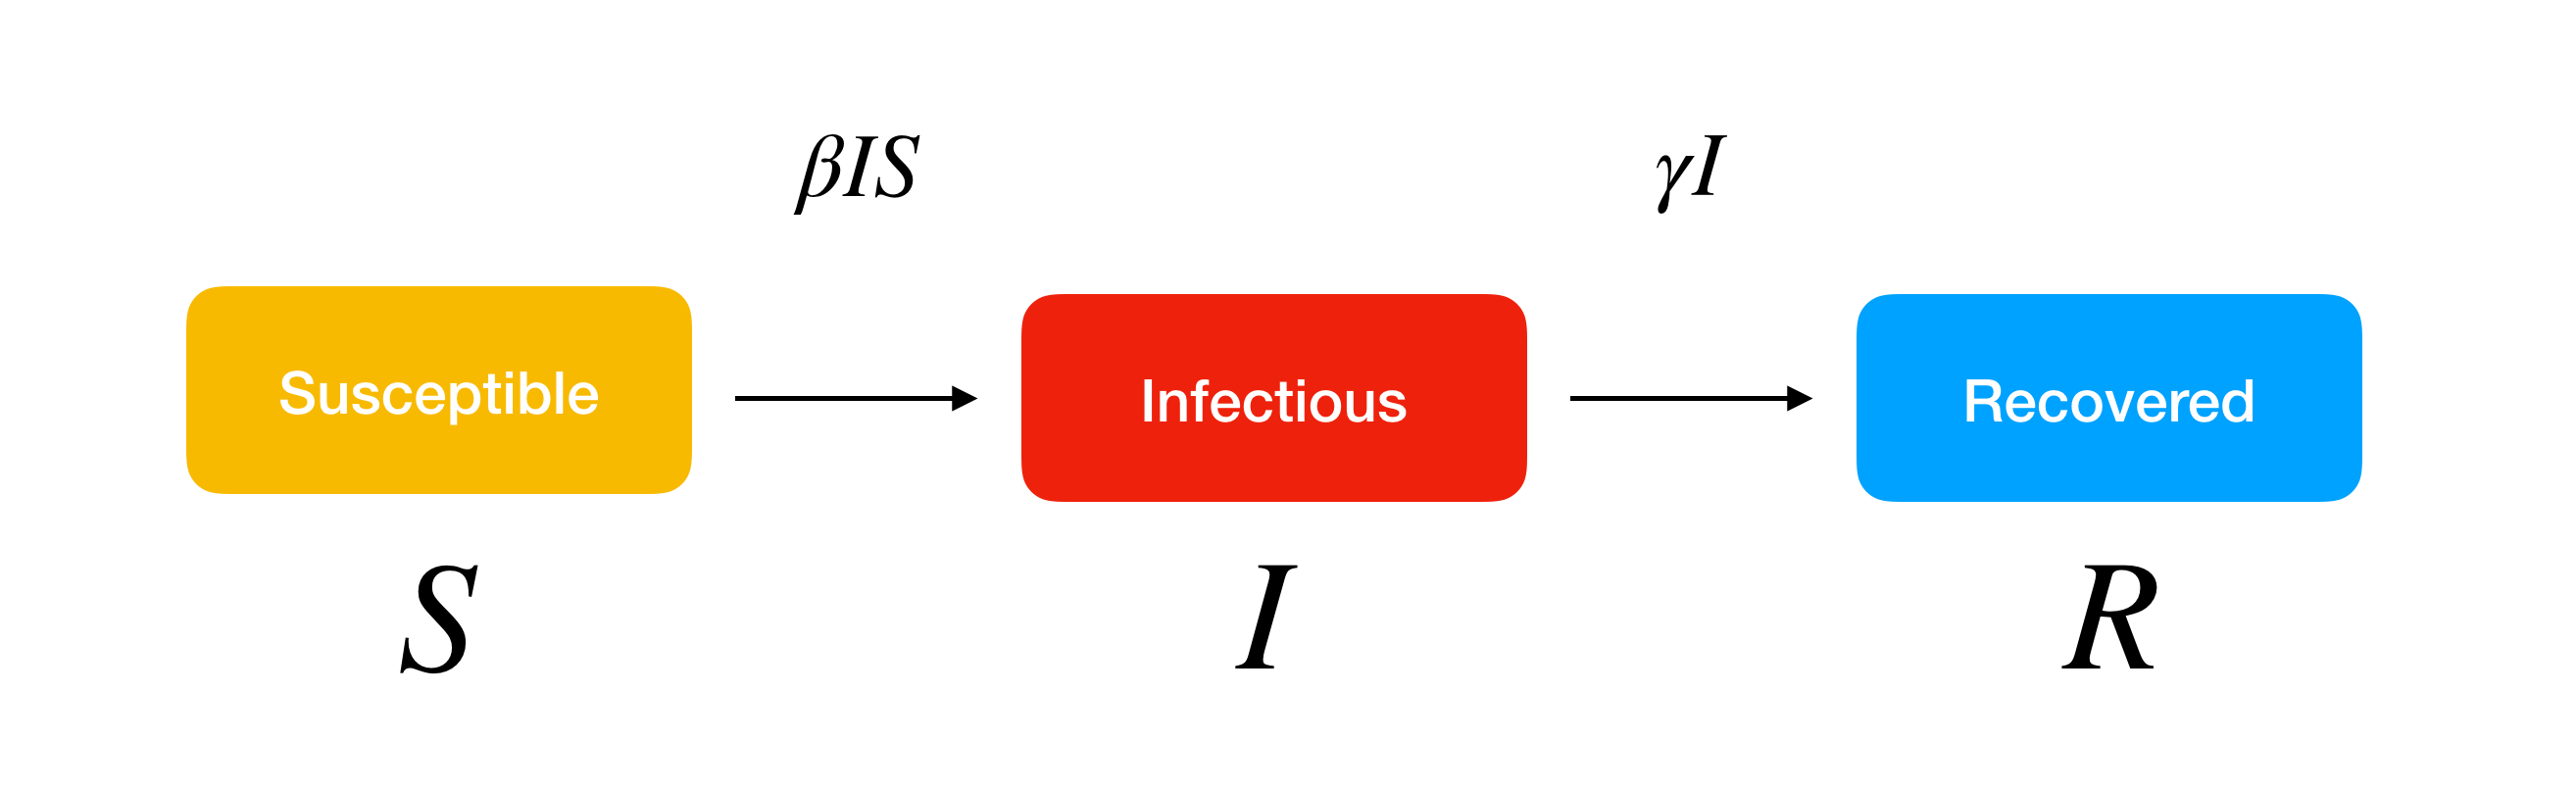
\includegraphics[width=9cm, height=3cm, center]{Images/sir.png}
        \caption{SIR MODEL}
        \label{fig:sir}
    \end{figure}
        \subsubsubsection*{Transition rates}
        \indent For the full specification of the model, the arrows should be labeled with the transition rates between compartments. Between $S$ and $I$, the transition rate is assumed to be $\frac{d(\frac{S}{N})}{dt} = \frac{- \beta SI}{N^2}$, where N is the total population, $\beta$ is the average number of contacts per person per time, multiplied by the probability of disease transmission in a contact between a susceptible and an infectious subject, and $\frac{SI}{N^2}$ is the fraction of those contacts between an infectious and susceptible individual which result in the susceptible person becoming infected. \\
        \indent Between $I$ and $R$, the transition rate is assumed to be proportional to the number of infectious individuals which is $\gamma I$. This is equivalent to assuming that the probability of an infectious individual recovering in any time interval dt is simply $\gamma dt$. If an individual is infectious for an average time period $D$, then $\gamma = \frac{1}{D}$. This is also equivalent to the assumption that the length of time spent by an individual in the infectious state is a random variable with an exponential distribution. The "classical" SIR model may be modified by using more complex and realistic distributions for the I-R transition rate.\\
        \indent For the special case in which there is no removal from the infectious compartment ($\gamma =0$), the SIR model reduces to a very simple SI model, which has a logistic solution, in which every individual eventually becomes infected.
        
\section{Exercises Part}
    \subsection{Exercise 1}
    \subsubsection{Discrete SIR Model}
        Assumptions: Assume that a type of flu is spreading within a community. We also assume that
        \begin{itemize}
            \item No one enters or leaves the community, and there is no contact outside the community.
            \item Each person is susceptible S (able to catch this new flu); infected I (currently has the flu and can spread the flu); or removed R (already had the flu and will not get it again, which includes death).
            \item Initially, every person is either S or I.
            \item Once someone gets the disease this year, they cannot get the disease again.
            \item The average length of the disease is 2 weeks, over which time the person is deemed infected and can spread the disease.
            \item Our time period for the model will be per week.
            \item The community is isolated.
            \item The recovery time of an infected individual is exactly 2 weeks and it does not change in time;
            \item Who recovered from the flu will be immune to it in the future;
            \item A susceptible individual becomes an infected individual with constant rate  ($\frac{\beta}{N}$). We also assume that the rate does not change in time.
        \end{itemize}
        Let’s assume the following definitions for our variables:
        \begin{itemize}
            \item $S(n)$ = number in the population susceptible after \textbf{period} $n$
            \item $I(n)$ =  number infected after \textbf{period} $n$
            \item $R(n)$ = number removed after \textbf{period} $n$
        \end{itemize}
        
        \indent Considering R(n), our assumption for the length of time someone has the flu is 2 weeks. Thus, 1/2 or 50\% of the infected people will be removed each week:
        \begin{align*}
            R(n+1) = R(n) + \gamma I= R(n) + 0.5I
        \end{align*}
        \indent The value $\gamma = 0.5$ is the \textit{removal rate per week}.It represents the proportion of the infected persons who are removed from infection each week. \\
        \indent I(n) will have terms that both increase and decrease its amount over time. It is decreased by the number of people removed each week: $0.5 * I(n)$. It is increased by the number of susceptible people who come into contact with infected people and catch the disease: $aS(n)I(n)$. We define $a$ as the rate at which the disease is spread, or the transmission coefficient. We realize this is a probabilistic coefficient. We will assume, initially, that this rate is a constant value that can be found from the initial conditions.\\
        \indent Let’s illustrate as follows: Assume we have a population of 1000 students residing in the dorms. Our nurse found 5 students reporting to the infirmary initially: I(0) = 5 and S(0) = 995. After one week, the total number infected with the flu is 11. We compute $a$ as follows:
        \begin{align*}
            I(0) & = 5, I(1) = I(0) - 0.5 I(0) + a I(0) S(0) \\
            I(1) & = 11 = 5 - 2.5 + a*5*995 \\
            a & = 0.001709
        \end{align*}  
        \indent Considering $S(n)$. This number is decreased only by the number that becomes infected.
        \begin{align*}
            S(n+1) = S(n) - a S(n) I(n)
        \end{align*}
        The SIR model is
        \begin{align*}
            R(n+1) & = R(n) + 0.5 I(n) \\
            I(n+1) & = I(n) - 0.5 I(n) + 0.001709 I(n) S(n) \\
            S(n+1) & = S(n) - 0.001709 S(n) I(n) \\
            S(0) & = 995,I(0) = 5,R(0) = 0 
        \end{align*}
        %%%%%%%%%%%%%%%%%%%%%%%%%%%%%%%%%%%%%%%%%%%%%%%%%
        
        \subsubsection{Continuous SIR Model}
        Assumptions: Assume that a type of flu is spreading within a community. We also assume that
        \begin{itemize}
            \item No one enters or leaves the community, and there is no contact outside the community.
            \item Each person is susceptible S (able to catch this new flu); infected I (currently has the flu and can spread the flu); or removed R (already had the flu and will not get it again, which includes death).
            \item Initially, every person is either S or I.
            \item Once someone gets the disease this year, they cannot get the disease again.
            \item The average length of the disease is 2 weeks, over which time the person is deemed infected and can spread the disease.
            \item Our time period for the model will be per week.
            \item The community is isolated.
            \item The recovery time of an infected individual is exactly 2 weeks and it does not change in time;
            \item Who recovered from the flu will be immune to it in the future;
            \item A susceptible individual becomes an infected individual with constant rate  ($\frac{\beta}{N}$). We also assume that the rate does not change in time.
        \end{itemize}
        
        Let’s assume the following definitions for our variables:
        \begin{itemize}
            \item $S(t)$ = number in the population susceptible after \textbf{time} $t$
            \item $I(t)$ =  number infected after \textbf{time} $t$
            \item $R(t)$ = number removed after \textbf{time} $t$
        \end{itemize}

        \indent Considering R(t), our assumption for the length of time someone has the flu is 2 weeks. Thus, 1/2 or 50\% of the infected people will be removed each week:
        \begin{align*}
            \frac{dR}{dt} = \gamma I(t)= 0.5I(t)
        \end{align*}
        
        \indent The value 0.5 is called the removal rate per week. The removal rate represents the proportion of the infected persons who are removed from infection each week. If real data are available, then we could do "data analysis" to obtain the removal rate. I(t) will have terms that both increase and decrease its amount over time. I(t) is decreased by the number removed each week, $0.5I(t)$. I(t) is increased by the number of susceptible who come into contact with an infected person and catch the disease, $aS(t)I(t)$. We define the rate $a$ as the rate at which the disease is spread, or the transmission coefficient. We realize this is a probabilistic coefficient. We will assume, initially, that this rate is a constant value that can be found from initial conditions. We use an estimate of 0.001709 for the rate $a$. \\
        \indent Considering S(t). This number is decreased only by the number who become infected. We may use the same rate a to obtain the model.
        \begin{align*}
            \frac{dS}{dt} = - \frac{\beta}{N} I(t) S(t) = - 0.001709I(t) S(t)
        \end{align*}
        \indent Our SIR model is shown in the following systems of differential equations:
        \begin{align*}
            \frac{dR}{dt} & = 0.5 I(t) \\
            \frac{dI}{dt} & = -0.5 I(t) + 0.001709 I(t) S(t) \\
            \frac{dS}{dt} & = 0.001709 S(t) I(t) \\
            S(0) & = 995,I(0) = 5,R(0) = 0 
        \end{align*}
        %%%%%%%%%%%%%%%%%%%%%%%%%%%%%%%%%%%%%%%%%%%%%%%%%
    \subsection{Exercise 2 - The RK4 method in solving the SIR system}
        \subsubsection{Preliminary}
        The most widely known member of the Runge–Kutta family is generally referred to as "RK4", the "classic Runge–Kutta method" or simply as "the Runge–Kutta method".RK4 is one of the classic methods for numerical integration of ODE models. \\
        Consider the following initial value problem of ODE 
        \begin{equation}\label{ODE}
            \begin{split}
                \frac{dy}{dt} & = f(t,y) \\ 
                 y(t_0) & = y_0
            \end{split}
        \end{equation}
        where y(t) is the unknown function (scalar or vector) which I would like to approximate.\\
        The iterative formula of RK4 method for solving ODE \eqref{ODE} is as follows
        \begin{equation}\label{RK4}
            \begin{split}
                y_{n+1} & = y_n + \frac{\Delta t}{6}(k_1 + 2k_2 + 2k_3 + k4) \\
                k_1 & = f(t_n,y_n) \\
                k_2 & = f(t_n + \frac{\Delta t}{2}, y_n + \frac{k_1 \Delta t}{2}) \\
                k_3 & = f(t_n + \frac{\Delta t}{2}, y_n + \frac{k_2 \Delta t}{2}) \\
                k_4 & = f(t_n + \Delta t, y_n + k_3 \Delta t) \\
                t_{n+1} & = t_n + \Delta t \\
                n & = 0,1,2,3,...
            \end{split}
        \end{equation}
        
        \indent The SIR model is defined as \eqref{1}, \eqref{2}, \eqref{3}. where S(t) is the number of susceptible people in the population at time t, I(t) is the number of infectious people at time t, R(t) is the number of recovered people at time t, $\beta$ is the transmission rate, $\gamma$ represents the recovery rate, and N=S(t)+I(t)+R(t) is the fixed population. \\
        \indent According to the general iterative formula \eqref{RK4}, the iterative formulas for S(t), I(t) and R(t) of SIR model can be written out. 
        \begin{figure}[h]
            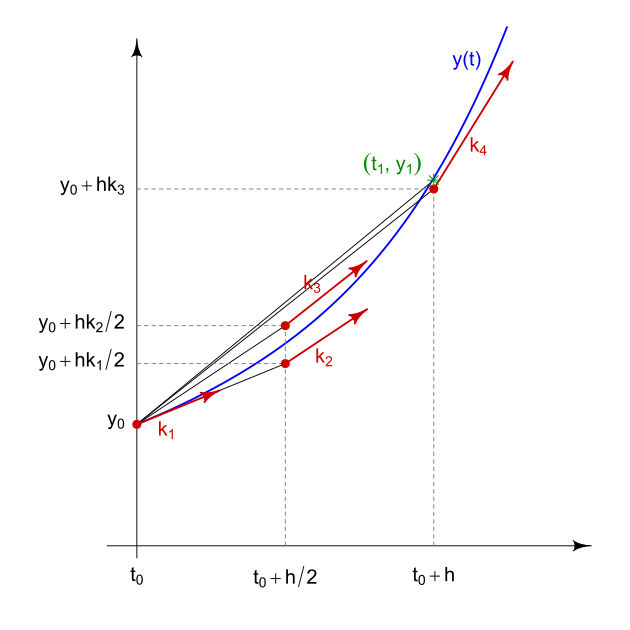
\includegraphics[width=10cm, height=9cm, center]{Images/Runge-Kutta_slopes.png}
            \caption{Slopes used by the classical Runge-Kutta method}
            \label{fig:rk4}
        \end{figure}
        \begin{equation}\label{RK4-SIR-1}
            \begin{split}
                S_{n+1} & = S_n + \frac{\Delta t}{6}(k_1^S + 2k_2^S + 2k_3^S + k4^S) \\
                k_1^S & = f(t_n,S_n, I_n) = - \frac{\beta S_n I_n}{N} \\
                k_2^S & = f(t_n + \frac{\Delta t}{2}, S_n + \frac{k_1^S \Delta t}{2}, I_n + \frac{k_1^I \Delta t}{2}) = -\frac{\beta}{N} ( S_n + \frac{k_1^S \Delta t}{2})(I_n + \frac{k_1^I \Delta t}{2})  \\
                k_3^S & = f(t_n + \frac{\Delta t}{2}, S_n + \frac{k_2^S \Delta t}{2}, I_n + \frac{k_2^I \Delta t}{2}) = -\frac{\beta}{N} ( S_n + \frac{k_2^S \Delta t}{2})(I_n + \frac{k_2^I \Delta t}{2})  \\
                k_4^S & = f(t_n + \Delta t, S_n + k_3^S \Delta t, I_n + k_3^I \Delta t) = -\frac{\beta}{N} (S_n + k_3^S \Delta t)(I_n + k_3^I \Delta t)
            \end{split}
        \end{equation}
        %%%%%%%%%%%%%%%%%%%%%%%%%%%%%%%%%%%%%
        \begin{equation}\label{RK4-SIR-2}
            \begin{split}
                I_{n+1} & = I_n + \frac{\Delta t}{6}(k_1^I+ 2k_2^I + 2k_3^I + k4^I) \\
                k_1^I & = f(t_n,S_n, I_n) = \frac{\beta S_n I_n}{N} - \gamma I_n \\
                k_2^I & = f(t_n + \frac{\Delta t}{2}, S_n + \frac{k_1^S \Delta t}{2}, I_n + \frac{k_1^I \Delta t}{2}) = \frac{\beta}{N} ( S_n + \frac{k_1^S \Delta t}{2})(I_n + \frac{k_1^I \Delta t}{2}) - \gamma (\frac{I_n + k_1^I \Delta t}{2})  \\
                k_3^I & = f(t_n + \frac{\Delta t}{2}, S_n + \frac{k_2^S \Delta t}{2}, I_n + \frac{k_2^I \Delta t}{2}) = \frac{\beta}{N} ( S_n + \frac{k_2^S \Delta t}{2})(I_n + \frac{k_2^I \Delta t}{2}) - \gamma (\frac{I_n + k_2^I \Delta t}{2})  \\
                k_4^I & = f(t_n + \Delta t, S_n + k_3^S \Delta t, I_n + k_3^I \Delta t) = \frac{\beta}{N} (S_n + k_3^S \Delta t)(I_n + k_3^I \Delta t) - \gamma (I_n + k_3^I \Delta t)
            \end{split}
        \end{equation}
        %%%%%%%%%%%%%%%%%%%%%%%%%%%%%%%%%%%%%
        \begin{equation}\label{RK4-SIR-3}
            \begin{split}
                R_{n+1} & = R_n + \frac{\Delta t}{6}(k_1^R + 2k_2^R + 2k_3^R + k_4^R) \\
                k_1^R & = f(t_n, I_n) = \gamma I_n \\
                k_2^R & = f(t_n + \frac{\Delta t}{2}, I_n + \frac{k_1^I \Delta t}{2}) = \gamma (\frac{I_n + k_1^I \Delta t}{2})  \\
                k_3^R & = f(t_n + \frac{\Delta t}{2}, I_n + \frac{k_2^I \Delta t}{2}) = \gamma (\frac{I_n + k_2^I \Delta t}{2})  \\
                k_4^R & = f(t_n + \Delta t, I_n + k_3^I \Delta t) = \gamma (I_n + k_3^I \Delta t)
            \end{split}
        \end{equation}
        \indent Note that since the population N = S(t) + I(t) + R(t) is constant, there will have $\frac{dS}{dt} + \frac{dI}{dt} + \frac{dr}{dt} = 0$. Therefore, only two of the three ODEs are independent and sufficient to solve the ODEs. Here, only iterative formulas for S(t) and I(t) are used and R(t) is calculated by S(t)=N - I(t) - R(t).
        
        \subsubsection{Implemetation}
        \subsubsubsection*{RK4 SIR Function}
        Firstly, I need to define some classes in order to make the code easier to imagine:
        \begin{itemize}
            \item \textbf{\textcolor{red}{SIRValue}} is used to store all the SIR input values including number of suspected, infected and recovered.
            \lstinputlisting[language=Python,firstline=11, lastline=32]{Implementations/Exercise2QuangRK4.py}
            
            \item \textbf{\textcolor{red}{SIRRatio}} is used to store all the input ratios including: $\beta$ - beta(contact rate) and $\gamma$ - gamma(recovery rate)
            \lstinputlisting[language=Python,firstline=35, lastline=38]{Implementations/Exercise2QuangRK4.py}
            
            \item \textbf{\textcolor{red}{Slop}} is used to store the SIRValue for futher calculation in other slops of RK4 (RK4 model needs to calculate 4 slops - $K1, K2, K3, K4$
            \lstinputlisting[language=Python,firstline=41, lastline=43]{Implementations/Exercise2QuangRK4.py}
            
            \item \textbf{\textcolor{red}{SIRRungeKuttaSlop}} is used to store all the \textbf{\textcolor{red}{Slop}}s to calculate the next RK4 value
            \lstinputlisting[language=Python,firstline=46, lastline=48]{Implementations/Exercise2QuangRK4.py}
        \end{itemize}
        
        Secondly, as the given SIR values are initial infected number $I_0$, initial recovered number $R_0$ and total population $N$. I need to implement:
        \begin{itemize}
            \item \textbf{\textcolor{red}{calculateSuspected}} function to calculate the suspected number:
            \lstinputlisting[language=Python,firstline=51, lastline=57]{Implementations/Exercise2QuangRK4.py}
            
            \item Moreover, as working on the helper functions of SIR, I also implement the \textbf{\textcolor{red}{printSIRValues}} function to print out the result in readable format:
            \lstinputlisting[language=Python,firstline=58, lastline=63]{Implementations/Exercise2QuangRK4.py}
        \end{itemize}
        
        Next, as RK4 model requires to evaluate the derivative of the value in the period of time $\Delta t$:
        \begin{itemize}
            \item Calculate the derivative of Suspected in the period of time by the function: $\frac{dS}{dt} = -\frac{\beta}{N}IS$
            \lstinputlisting[language=Python,firstline=74, lastline=85]{Implementations/Exercise2QuangRK4.py}
            
            \item Calculate the derivative of Infected in the period of time by the function: $\frac{dI}{dt} = \frac{\beta}{N}IS - {\gamma} I$
            \lstinputlisting[language=Python,firstline=89, lastline=94]{Implementations/Exercise2QuangRK4.py}
            
            \item Calculate the derivative of Recovered in the period of time by the function: $\frac{dS}{dt} = {\gamma} I$
            \lstinputlisting[language=Python,firstline=98, lastline=103]{Implementations/Exercise2QuangRK4.py}
        \end{itemize}
        
        In the next step, we implement the Runge Kutta model's helper functions in order to calculate the slop more easyly:
        \begin{itemize}
            \item \textbf{\textcolor{red}{calculateSlopValues}} function is used to evaluate the differential values of the slop
            \lstinputlisting[language=Python,firstline=108, lastline=113]{Implementations/Exercise2QuangRK4.py}
            
            \item \textbf{\textcolor{red}{calculateInitialSlop}} function is used to evaluate the first slop of RK4 by the given RK4 function: ${k_1} = f(t_n, y_n)$
            \lstinputlisting[language=Python,firstline=121, lastline=130]{Implementations/Exercise2QuangRK4.py}
            
            \item \textbf{\textcolor{red}{calculateMiddleSlop}} function is used to evaluate the second and third slop of RK4 by the given RK4 function: ${k_2} = f(t_n + \frac{\Delta t}{2}, y_n + \frac{\Delta t}{2}k_1)$ , ${k_3} = f(t_n + \frac{\Delta t}{2}, y_n + \frac{\Delta t}{2}k_2)$
            \lstinputlisting[language=Python,firstline=137, lastline=161]{Implementations/Exercise2QuangRK4.py}
            
            \item \textbf{\textcolor{red}{calculateLastSlop}} function is used to evaluate the last slop of RK4 by the given RK4 function: ${k_4} = f(t_n + {\Delta t}, y_n + {\Delta t}k_1)$
            \lstinputlisting[language=Python,firstline=167, lastline=192]{Implementations/Exercise2QuangRK4.py}
        \end{itemize}
        
            In the last and final step, we need to implement the \textbf{\textcolor{blue}{Runge Kutta - SIR}} model functions to take in the inputs and calculate the logic of the Runge Kutta method: 
        
        \begin{itemize}
            \item \textbf{\textcolor{red}{approximateRK4SIR}} function is used to evaluate all slops of the Runge Kutta method and all the SIR values in the given period of time $\Delta t$.
            \lstinputlisting[language=Python,firstline=205, lastline=259]{Implementations/Exercise2QuangRK4.py}
            
            \item \textbf{\textcolor{red}{RK4SIR}} function is used to handle all the inputs and triggers the logic of Runge Kutta function to execute. 
            \lstinputlisting[language=Python,firstline=263, lastline=271]{Implementations/Exercise2QuangRK4.py}
        \end{itemize}
        %figure plot RK4
        Then to test if the RK4SIR function is actually working we need to implement the ploting machanizm in order to visualize the SIR model using graphic.
        \\
        \emph{\textcolor{cyan}{This is how we implement the plotting}}
        \lstinputlisting[language=Python, firstline=274, lastline=301]{Implementations/Exercise2QuangRK4.py}
        
        \emph{And this is the result of the plot with $\beta = 2, \gamma = 0.5, N = 1000, I_0 = 1, R_0 =1$}
        \begin{figure}[h!]
            \centering
            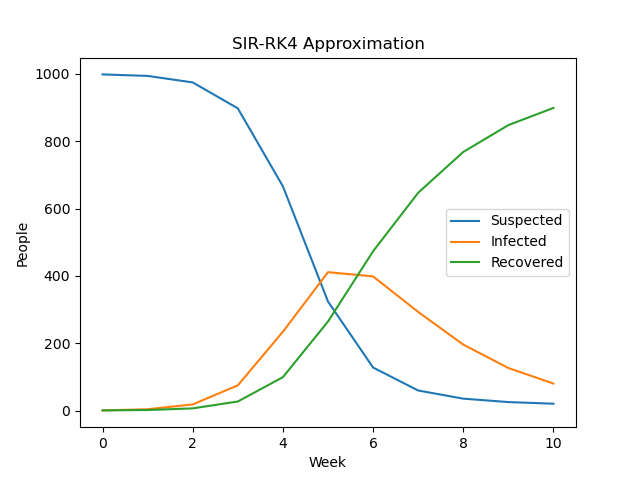
\includegraphics[width=1\linewidth]{Images/plotRK4.png}
            \caption*{Plotting with $\beta = 2, \gamma = 0.5, N = 1000, I_0 = 1, R_0 =1$}
        \end{figure}

    \subsection{Exercise 3}
    \subsubsection{Background}
    The Metropolis–Hastings algorithm can be used to take random samples from any probability distribution. Provied that we know a function f(x) that is atleast propotional to the original probability density function.
    \\
    In this problem, we will consider taking sample of the parameter $\beta$ and $\gamma$ in the SIR model the prior from distribution $\pi(\beta, \gamma)$. Assuming $\beta$ and $\gamma$ are indepentdent, we have:
    \begin{align*}
        \pi(\beta, \gamma) = \pi(\beta).\pi( \gamma)
    \end{align*}
    Where $\pi(\beta)$ is the prior distribution of $\beta$ and $\pi(\gamma)$ is the prior distribution $\gamma$
    \\
    Sample draws from this distribution will be used later on in excersice 4 along with real data regarding covid-19. Therefore, we need to give a reasonable guess about the prior distribution of $\beta$ and $\gamma$
    \\
    \indent For $\beta$ - the tranmission rate under SIR model. In the case of covid-19 disease, this rate is not easy to estimate and the result varied a lot from region to region as well as it's also depending alot on social distancing policies. Therfore, we'll assume that it has a prior uniform distribution $U(10^{-3}, 6)$, meaning that $\beta$ can have an equal chance of having any value between $10^{-3}$ and $6$.
    \\
    \indent For $\gamma$ - the recovering rate under SIR model. It's reasonable to let it be the inverse of the disease recovering time. For example, with the average recovering time of covid-19 being 2 weeks, $\gamma$ should have an expected value of 1/14. Or in other words, one over fourteen of the infected group will recover per day. With this in mind, we can let $\gamma$ follow the normal distribution $N(1/14, 0.1/14)$. Most of the value of $\gamma$ in this distribution is in the range of 1/28 to 3/28, corresponding to an estimated recovering time from 1.33 weeks to 4 weeks, which fit nicely with real recovering time of covid-19.
    \\
    In this assignment, we will construct our own Metropolis-Hastings algorithm that will perform the following steps:
    \\
    \indent 1. Initialize $\beta_0$ and $\gamma_0$.
    \\
    \indent 2. Set $\beta$ := $\beta_0$ and $\gamma$ := $\gamma_0$.
    \\
    \indent 3. Select the next $\beta*$ and $\gamma*$ using current $\beta, \gamma$ randomly from $Q(\beta, \gamma)$. Namely, we choose this proposal distribution to be comprised of two probability distribution $N(\beta, \sigma_1)$ and $N(\gamma, \sigma_2)$. Where $\sigma_1$ and $\sigma_2$ are constansts that can be adjusted to better fit our prior distribution.
    \\
    \indent 4. Calculated the ratio that'll tell us how likely the new $\beta*$ and $\gamma*$ fit the original distribution compared to the current ones
    \begin{align*}
        r = \frac{\pi(\beta*, \gamma*)Q(\beta, \gamma|\beta*, \gamma*)}{\pi(\beta, \gamma)Q(\beta*, \gamma*|\beta, \gamma)}
    \end{align*}
    
    Note: because we choose our transistion model to follow a Normal distribution with constant variance, $Q(\beta, \gamma|\beta*, \gamma*)$ will be equal to $Q(\beta*, \gamma*|\beta, \gamma)$ because this is a symmertric distribution.
    \\
    \indent 5. Generate a value $\alpha$ randomly from a continuous uniform distribution U(0; 1).
    \\
    \indent 6. If $\alpha$ < r, set $\beta_{i+1}$ := $\beta*$ and $\gamma_{i+1}$ := $\gamma*$, and move to Step 8.
    \\
    \indent 7. Otherwise, set $\beta_{i+1}$ := $\beta_i$ and $\gamma_{i+1}$ := $\gamma_i$, and move to Step 8.
    \\
    \indent 8. Repeat Step 2 with $\beta$ := $\beta_{i+1}$ and $\gamma$ := $\gamma_{i+1}$ until we get m elements.
    \subsubsection{Implementation}
    Implementing Metropolis-Hasting algorithm as a helper function to support calculating the prior sampling in file: "Ex3libMHSimplified.py".   
    \lstinputlisting[language=Python]{Implementations/Ex3libMHSimplified.py}
    Calling the MH function and passing the right probability functions:
    \lstinputlisting[language=Python, firstline=1, lastline=42]{Implementations/Ex3_PriorSampling.py}
    Plotting the trace and sampling process from MH return results:
    \lstinputlisting[language=Python, firstline=43, lastline=123]{Implementations/Ex3_PriorSampling.py}
    
    Run this exercise with library "matplotlib","numby", required python 3 package, 2 file "Ex3libMHSimplified.py","Ex3PriorSampling.py" in the same directory.
    \begin{enumerate}
        \item Open Command Promt then enter "python Ex3-PriorSampling.py"
        \item Enter m: 10000
        \item Enter sigma1: 1.73
        \item Enter sigma2: 0.014 ($\frac{1}{70}$)
        \item Enter burnIn: 3000
    \end{enumerate}
    Results: the first one show the sampling procress happend all along 10000 iteration, the second show the process of the first 1000 iteration
    \begin{figure}[!ht]
        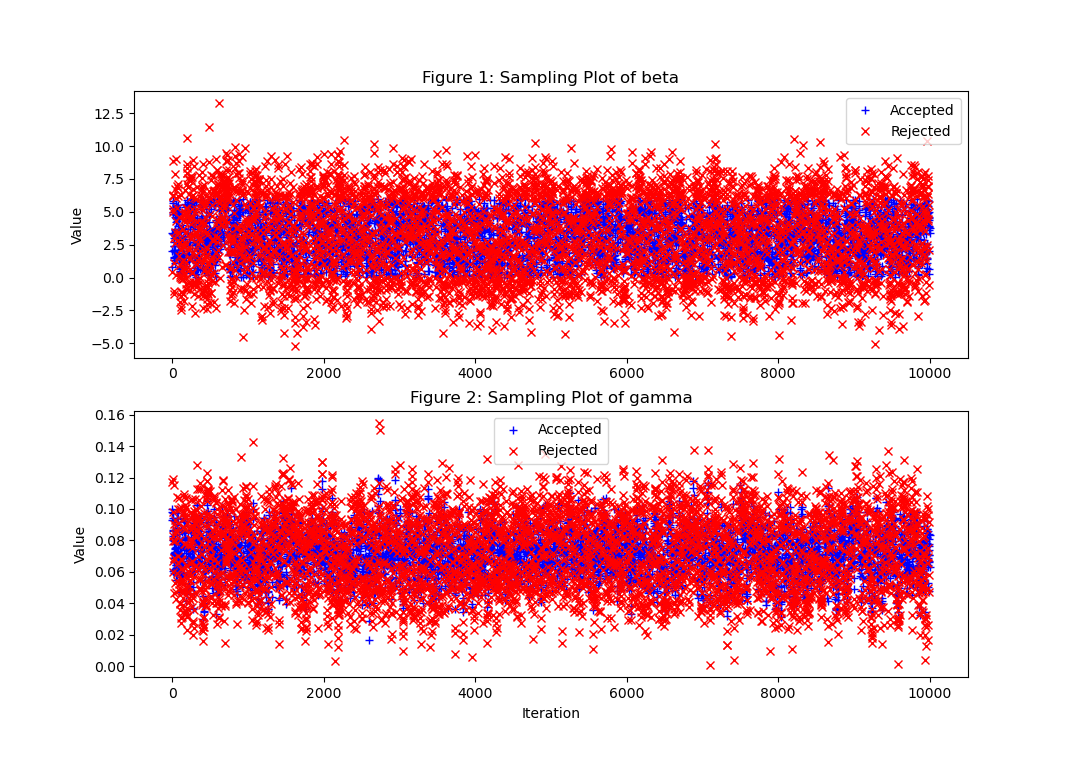
\includegraphics[width=\linewidth, inner]{Images/ex3plot1.png}
        \caption{Plot 1}
        \label{fig:ex3-1}
    \end{figure}
    \newpage
    \begin{figure}[!ht]
        \centering
        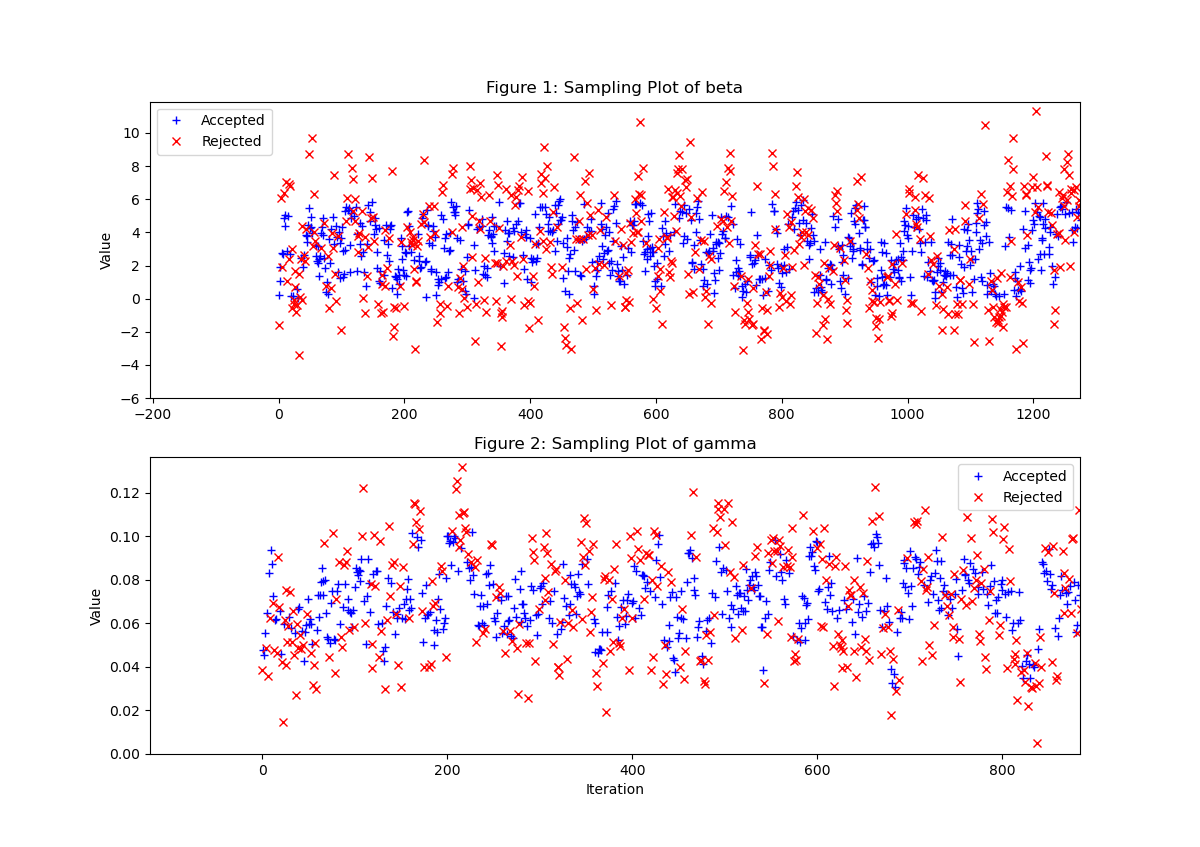
\includegraphics[width=\linewidth]{Images/ex3plot1000.png}
        \caption{1000 iteration}
        \label{fig:ex3-2}
    \end{figure}
    \begin{figure}[!ht]
        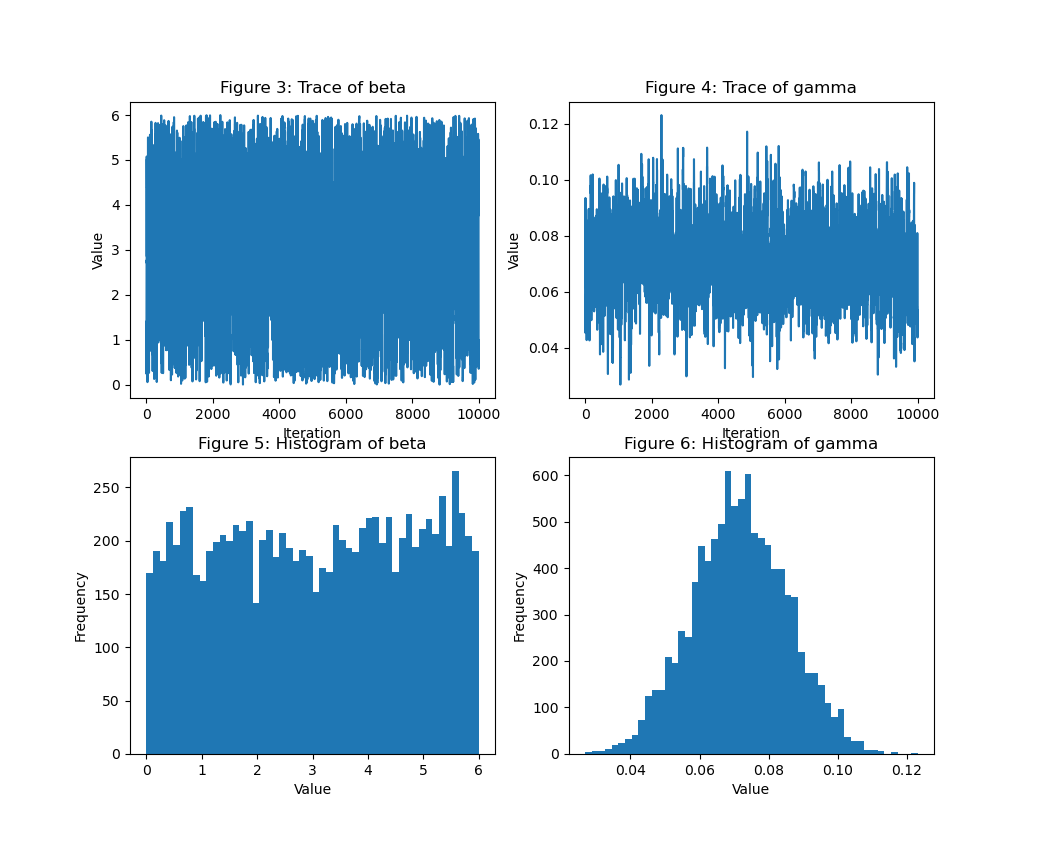
\includegraphics[width=\linewidth, inner]{Images/ex3plot2.png}
        \caption{Plot 2}
        \label{fig:ex3-3}
    \end{figure}

    \subsection{Craw data for Exercise 4}
    %%%%%%%%%%%%%%%%%%%%%%%%%%%%%%%

    \begin{tcolorbox}[breakable, size=fbox, boxrule=1pt, pad at break*=1mm,colback=cellbackground, colframe=cellborder]
\prompt{In}{incolor}{36}{\boxspacing}
\begin{Verbatim}[commandchars=\\\{\}]
\PY{n}{EU\PYZus{}nation} \PY{o}{=} \PYZbs{}
\PY{l+s+sd}{\PYZdq{}\PYZdq{}\PYZdq{}\PYZbs{}}
\PY{l+s+sd}{Austria, Belgium, Bulgaria, Croatia, Cyprus, \PYZbs{}}
\PY{l+s+sd}{Czechia, Denmark, Estonia, Finland, France, Germany,\PYZbs{}}
\PY{l+s+sd}{Greece, Hungary, Ireland, Italy, Latvia, Lithuania, Luxembourg,\PYZbs{}}
\PY{l+s+sd}{Malta, Netherlands, Poland, Portugal, Romania, \PYZbs{}}
\PY{l+s+sd}{Slovakia, Slovenia, Spain, Sweden \PYZbs{}}
\PY{l+s+sd}{\PYZdq{}\PYZdq{}\PYZdq{}}\PY{o}{.}\PY{n}{replace}\PY{p}{(}\PY{l+s+s2}{\PYZdq{}}\PY{l+s+s2}{ }\PY{l+s+s2}{\PYZdq{}}\PY{p}{,}\PY{l+s+s2}{\PYZdq{}}\PY{l+s+s2}{\PYZdq{}}\PY{p}{)}\PY{o}{.}\PY{n}{split}\PY{p}{(}\PY{l+s+s2}{\PYZdq{}}\PY{l+s+s2}{,}\PY{l+s+s2}{\PYZdq{}}\PY{p}{)}

\PY{c+c1}{\PYZsh{} United Kingdom did not official exit from the EU}
\PY{c+c1}{\PYZsh{} so we still consider UK is a part of EU}

\PY{n}{EU\PYZus{}nation}\PY{o}{.}\PY{n}{append}\PY{p}{(}\PY{l+s+s1}{\PYZsq{}}\PY{l+s+s1}{United Kingdom}\PY{l+s+s1}{\PYZsq{}}\PY{p}{)}

\PY{n}{EU\PYZus{}poplation} \PY{o}{=} \PY{n}{EU\PYZus{}poplation}\PY{p}{[}\PY{n}{EU\PYZus{}poplation}\PY{p}{[}\PY{l+s+s1}{\PYZsq{}}\PY{l+s+s1}{Name}\PY{l+s+s1}{\PYZsq{}}\PY{p}{]}\PY{o}{.}\PY{n}{isin}\PY{p}{(}\PY{n}{EU\PYZus{}nation}\PY{p}{)}\PY{p}{]}\PY{o}{.}\PYZbs{}
                \PY{n}{reset\PYZus{}index}\PY{p}{(}\PY{n}{drop}\PY{o}{=}\PY{k+kc}{True}\PY{p}{)}
\end{Verbatim}
\end{tcolorbox}

    
    
    %%%%%%%%%%%%%%%%%%%%%%%%%%%%%%%
    \subsubsection{Get EU Case}

    \hypertarget{john-hopskin-corona-virus-repository}{%
\subsubsubsection*{JOHN HOPSKIN Corona-Virus
Repository}\label{john-hopskin-corona-virus-repository}}

    We use data from
COVID-19/csse\_covid\_19\_data/csse\_covid\_19\_time\_series/ that was
cloned from https://github.com/CSSEGISandData/COVID-19 in 08/07/2020

This folder contains daily time series summary tables, including
confirmed, deaths and recovered. All data is read in from the daily case
report. The time series tables are subject to be updated if inaccuracies
are identified in our historical data. The daily reports will not be
adjusted in these instances to maintain a record of raw data.

Two time series tables are for the US confirmed cases and deaths,
reported at the county level. They are named
time\_series\_covid19\_confirmed\_US.csv,
time\_series\_covid19\_deaths\_US.csv, respectively.

Three time series tables are for the global confirmed cases, recovered
cases and deaths. Australia, Canada and China are reported at the
province/state level. Dependencies of the Netherlands, the UK, France
and Denmark are listed under the province/state level. The US and other
countries are at the country level. The tables are renamed
time\_series\_covid19\_confirmed\_global.csv and
time\_series\_covid19\_deaths\_global.csv, and
time\_series\_covid19\_recovered\_global.csv, respectively.

    \textbf{General Information}\label{general-information}

    We decide to use 3 data file:

\begin{itemize}
\tightlist
\item
  TIME\_SERIES\_COVID19\_CONFIRMED\_GLOBAL\_CSV
\item
  TIME\_SERIES\_COVID19\_RECOVERED\_GLOBAL\_CSV\_PATH
\item
  TIME\_SERIES\_COVID19\_DEATHS\_GLOBAL\_CSV\_PATH
\end{itemize}

Those files share some simlarites:

The Data about Corona-Virus from the JOHN HOPSKIN is contain the data
from more than 173 Countries/Regions recorded from 1/22/20 to 7/8/20
(MM/DD/YY) in the time, we cloned to our repos.

Only have Null value at the Province/State, which is reasonable.

    \begin{tcolorbox}[breakable, size=fbox, boxrule=1pt, pad at break*=1mm,colback=cellbackground, colframe=cellborder]
\prompt{In}{incolor}{13}{\boxspacing}
\begin{Verbatim}[commandchars=\\\{\}]
\PY{n}{dat\PYZus{}confirmed} \PY{o}{=} \PY{n}{data\PYZus{}process}\PY{o}{.}\PY{n}{read\PYZus{}csv}\PY{p}{(}\PY{n}{file\PYZus{}path}\PY{p}{[}\PYZbs{}
                    \PY{l+s+s1}{\PYZsq{}}\PY{l+s+s1}{TIME\PYZus{}SERIES\PYZus{}COVID19\PYZus{}CONFIRMED\PYZus{}GLOBAL\PYZus{}CSV\PYZus{}PATH}\PY{l+s+s1}{\PYZsq{}}\PY{p}{]}\PY{p}{)}
\end{Verbatim}
\end{tcolorbox}

    \begin{tcolorbox}[breakable, size=fbox, boxrule=1pt, pad at break*=1mm,colback=cellbackground, colframe=cellborder]
\prompt{In}{incolor}{71}{\boxspacing}
\begin{Verbatim}[commandchars=\\\{\}]
\PY{n}{dat\PYZus{}recovered} \PY{o}{=} \PY{n}{data\PYZus{}process}\PY{o}{.}\PY{n}{read\PYZus{}csv}\PY{p}{(}\PY{n}{file\PYZus{}path}\PY{p}{[}\PYZbs{}
                    \PY{l+s+s1}{\PYZsq{}}\PY{l+s+s1}{TIME\PYZus{}SERIES\PYZus{}COVID19\PYZus{}RECOVERED\PYZus{}GLOBAL\PYZus{}CSV\PYZus{}PATH}\PY{l+s+s1}{\PYZsq{}}\PY{p}{]}\PY{p}{)}
\end{Verbatim}
\end{tcolorbox}

    \begin{tcolorbox}[breakable, size=fbox, boxrule=1pt, pad at break*=1mm,colback=cellbackground, colframe=cellborder]
\prompt{In}{incolor}{72}{\boxspacing}
\begin{Verbatim}[commandchars=\\\{\}]
\PY{n}{dat\PYZus{}death} \PY{o}{=} \PY{n}{data\PYZus{}process}\PY{o}{.}\PY{n}{read\PYZus{}csv}\PY{p}{(}\PY{n}{file\PYZus{}path}\PY{p}{[}\PYZbs{}
                    \PY{l+s+s1}{\PYZsq{}}\PY{l+s+s1}{TIME\PYZus{}SERIES\PYZus{}COVID19\PYZus{}DEATHS\PYZus{}GLOBAL\PYZus{}CSV\PYZus{}PATH}\PY{l+s+s1}{\PYZsq{}}\PY{p}{]}\PY{p}{)}
\end{Verbatim}
\end{tcolorbox}

    %%%%%%%%%%%%%%%%%%%%%%%%%%%%%%%
    \subsubsection{EU General Analysis}
    
    \begin{center}
    \adjustimage{max size={0.9\linewidth}{0.9\paperheight}}{Images/crawlPlot1.png}
    \end{center}
    { \hspace*{\fill} \\}
    
    \textbf{EU COVID-19 case on 07/08/2020}

    \begin{tcolorbox}[breakable, size=fbox, boxrule=1pt, pad at break*=1mm,colback=cellbackground, colframe=cellborder]
\prompt{In}{incolor}{57}{\boxspacing}
\begin{Verbatim}[commandchars=\\\{\}]
\PY{n}{EU\PYZus{}07\PYZus{}08\PYZus{}2020} \PY{o}{=} \PY{n}{EU\PYZus{}confirmed}\PY{p}{[}\PY{p}{[}\PY{l+s+s1}{\PYZsq{}}\PY{l+s+s1}{Country/Region}\PY{l+s+s1}{\PYZsq{}}\PY{p}{,}\PY{l+s+s1}{\PYZsq{}}\PY{l+s+s1}{7/8/20}\PY{l+s+s1}{\PYZsq{}}\PY{p}{]}\PY{p}{]}

\PY{n}{EU\PYZus{}07\PYZus{}08\PYZus{}2020} \PY{o}{=} \PY{n}{EU\PYZus{}07\PYZus{}08\PYZus{}2020}\PY{o}{.}\PY{n}{rename}\PY{p}{(}\PY{n}{columns}\PY{o}{=}\PY{p}{\PYZob{}}\PY{l+s+s1}{\PYZsq{}}\PY{l+s+s1}{7/8/20}\PY{l+s+s1}{\PYZsq{}}\PY{p}{:}\PY{l+s+s1}{\PYZsq{}}\PY{l+s+s1}{Confirmed}\PY{l+s+s1}{\PYZsq{}}\PY{p}{\PYZcb{}}\PY{p}{)}

\PY{n}{EU\PYZus{}07\PYZus{}08\PYZus{}2020} \PY{o}{=} \PY{n}{pd}\PY{o}{.}\PY{n}{concat}\PY{p}{(}\PY{p}{[}\PY{n}{EU\PYZus{}07\PYZus{}08\PYZus{}2020}\PY{p}{,} \PY{n}{EU\PYZus{}recover}\PY{p}{[}\PY{l+s+s1}{\PYZsq{}}\PY{l+s+s1}{7/8/20}\PY{l+s+s1}{\PYZsq{}}\PY{p}{]}\PY{p}{]}\PY{p}{,} \PY{n}{axis} \PY{o}{=}\PY{l+m+mi}{1}\PY{p}{)}

\PY{n}{EU\PYZus{}07\PYZus{}08\PYZus{}2020} \PY{o}{=} \PY{n}{EU\PYZus{}07\PYZus{}08\PYZus{}2020}\PY{o}{.}\PY{n}{rename}\PY{p}{(}\PY{n}{columns}\PY{o}{=}\PY{p}{\PYZob{}}\PY{l+s+s1}{\PYZsq{}}\PY{l+s+s1}{7/8/20}\PY{l+s+s1}{\PYZsq{}}\PY{p}{:}\PY{l+s+s1}{\PYZsq{}}\PY{l+s+s1}{Recover}\PY{l+s+s1}{\PYZsq{}}\PY{p}{\PYZcb{}}\PY{p}{)}

\PY{n}{EU\PYZus{}07\PYZus{}08\PYZus{}2020} \PY{o}{=} \PY{n}{pd}\PY{o}{.}\PY{n}{concat}\PY{p}{(}\PY{p}{[}\PY{n}{EU\PYZus{}07\PYZus{}08\PYZus{}2020}\PY{p}{,} \PY{n}{EU\PYZus{}death}\PY{p}{[}\PY{l+s+s1}{\PYZsq{}}\PY{l+s+s1}{7/8/20}\PY{l+s+s1}{\PYZsq{}}\PY{p}{]}\PY{p}{]}\PY{p}{,} \PY{n}{axis} \PY{o}{=}\PY{l+m+mi}{1}\PY{p}{)}

\PY{n}{EU\PYZus{}07\PYZus{}08\PYZus{}2020} \PY{o}{=} \PY{n}{EU\PYZus{}07\PYZus{}08\PYZus{}2020}\PY{o}{.}\PY{n}{rename}\PY{p}{(}\PY{n}{columns}\PY{o}{=}\PY{p}{\PYZob{}}\PY{l+s+s1}{\PYZsq{}}\PY{l+s+s1}{7/8/20}\PY{l+s+s1}{\PYZsq{}}\PY{p}{:}\PY{l+s+s1}{\PYZsq{}}\PY{l+s+s1}{Death}\PY{l+s+s1}{\PYZsq{}}\PY{p}{\PYZcb{}}\PY{p}{)}

\PY{n}{EU\PYZus{}07\PYZus{}08\PYZus{}2020}\PY{o}{.}\PY{n}{set\PYZus{}index}\PY{p}{(}\PY{l+s+s1}{\PYZsq{}}\PY{l+s+s1}{Country/Region}\PY{l+s+s1}{\PYZsq{}}\PY{p}{,}\PY{n}{inplace} \PY{o}{=} \PY{k+kc}{True}\PY{p}{)}
\end{Verbatim}
\end{tcolorbox}

    As we review the data, some countries actually do not have the actual
number of recovered case, So we decide to remove :

\begin{itemize}
\tightlist
\item
  United Kingdom
\item
  Sweden
\item
  Netherlands
\end{itemize}

Due to the large different in number of cases between country, we will
choose country that had more than 5000 confirmed cases on 07/08/2020

    \begin{tcolorbox}[breakable, size=fbox, boxrule=1pt, pad at break*=1mm,colback=cellbackground, colframe=cellborder]
\prompt{In}{incolor}{58}{\boxspacing}
\begin{Verbatim}[commandchars=\\\{\}]
\PY{n}{EU\PYZus{}07\PYZus{}08\PYZus{}2020}\PY{o}{.}\PY{n}{plot}\PY{o}{.}\PY{n}{bar}\PY{p}{(}\PY{n}{figsize} \PY{o}{=}\PY{p}{[}\PY{l+m+mi}{12}\PY{p}{,}\PY{l+m+mi}{9}\PY{p}{]}\PY{p}{)}
\end{Verbatim}
\end{tcolorbox}
        
    \begin{center}
    \adjustimage{max size={0.9\linewidth}{0.9\paperheight}}{Images/crawlPlot2.png}
    \end{center}
    { \hspace*{\fill} \\}
    
    \begin{tcolorbox}[breakable, size=fbox, boxrule=1pt, pad at break*=1mm,colback=cellbackground, colframe=cellborder]
\prompt{In}{incolor}{59}{\boxspacing}
\begin{Verbatim}[commandchars=\\\{\}]
\PY{n}{EU\PYZus{}07\PYZus{}08\PYZus{}2020}\PY{o}{.}\PY{n}{drop}\PY{p}{(}\PY{p}{[}\PY{l+s+s1}{\PYZsq{}}\PY{l+s+s1}{United Kingdom}\PY{l+s+s1}{\PYZsq{}}\PY{p}{,}\PY{l+s+s1}{\PYZsq{}}\PY{l+s+s1}{Sweden}\PY{l+s+s1}{\PYZsq{}}\PY{p}{,}\PY{l+s+s1}{\PYZsq{}}\PY{l+s+s1}{Netherlands}\PY{l+s+s1}{\PYZsq{}}\PY{p}{]}\PY{p}{,}
                   \PY{n}{inplace} \PY{o}{=}\PY{k+kc}{True}\PY{p}{)}

\PY{n}{EU\PYZus{}07\PYZus{}08\PYZus{}2020} \PY{o}{=} \PY{n}{EU\PYZus{}07\PYZus{}08\PYZus{}2020}\PY{p}{[}\PY{n}{EU\PYZus{}07\PYZus{}08\PYZus{}2020}\PY{p}{[}\PY{l+s+s1}{\PYZsq{}}\PY{l+s+s1}{Confirmed}\PY{l+s+s1}{\PYZsq{}}\PY{p}{]} \PY{o}{\PYZgt{}} \PY{l+m+mi}{5000}\PY{p}{]}

\PY{n}{EU\PYZus{}07\PYZus{}08\PYZus{}2020}\PY{o}{.}\PY{n}{plot}\PY{o}{.}\PY{n}{bar}\PY{p}{(}\PY{n}{figsize} \PY{o}{=}\PY{p}{[}\PY{l+m+mi}{12}\PY{p}{,}\PY{l+m+mi}{9}\PY{p}{]}\PY{p}{)}
\end{Verbatim}
\end{tcolorbox}


    %%%%%%%%%%%%%%%%%%%%%%%%%%%%%%%
    \subsubsection{Processed daily cases}
    
    \textbf{Calculate new case daily}\label{calculate-new-case-daily}

    For some unknown reasons, The newly case update fall below 0, which does
not make any sense.

    \begin{tcolorbox}[breakable, size=fbox, boxrule=1pt, pad at break*=1mm,colback=cellbackground, colframe=cellborder]
\prompt{In}{incolor}{13}{\boxspacing}
\begin{Verbatim}[commandchars=\\\{\}]
\PY{k}{for} \PY{n}{df\PYZus{}name}\PY{p}{,} \PY{n}{df} \PY{o+ow}{in} \PY{p}{[}\PY{p}{[}\PY{l+s+s1}{\PYZsq{}}\PY{l+s+s1}{daily\PYZus{}confirmed}\PY{l+s+s1}{\PYZsq{}}\PY{p}{,} \PY{n}{confirmed}\PY{p}{]}\PY{p}{,}
                    \PY{p}{[}\PY{l+s+s1}{\PYZsq{}}\PY{l+s+s1}{daily\PYZus{}recovered}\PY{l+s+s1}{\PYZsq{}}\PY{p}{,} \PY{n}{recovered}\PY{p}{]}\PY{p}{,}
                    \PY{p}{[}\PY{l+s+s1}{\PYZsq{}}\PY{l+s+s1}{daily\PYZus{}death}\PY{l+s+s1}{\PYZsq{}}\PY{p}{,} \PY{n}{death}\PY{p}{]}\PY{p}{]}\PY{p}{:}

    \PY{n}{nations} \PY{o}{=} \PY{n}{df}\PY{o}{.}\PY{n}{columns}\PY{p}{[}\PY{l+m+mi}{1}\PY{p}{:}\PY{p}{]}
    
    \PY{n}{new\PYZus{}daily\PYZus{}case} \PY{o}{=} \PY{n}{df}\PY{p}{[}\PY{p}{[}\PY{l+s+s1}{\PYZsq{}}\PY{l+s+s1}{Date}\PY{l+s+s1}{\PYZsq{}}\PY{p}{]}\PY{p}{]}\PY{p}{[}\PY{p}{:}\PY{o}{\PYZhy{}}\PY{l+m+mi}{1}\PY{p}{]}

    \PY{k}{for} \PY{n}{nation} \PY{o+ow}{in} \PY{n}{nations}\PY{p}{:}

        \PY{n}{new\PYZus{}daily\PYZus{}case}\PY{p}{[}\PY{n}{nation}\PY{p}{]} \PY{o}{=} \PY{n}{get\PYZus{}new\PYZus{}daily\PYZus{}case}\PY{p}{(}\PY{n}{df}\PY{p}{,} \PY{n}{nation}\PY{p}{)}
        
    \PY{n}{ix\PYZus{}below\PYZus{}zero} \PY{o}{=} \PY{n}{np}\PY{o}{.}\PY{n}{where}\PY{p}{(}\PY{n}{new\PYZus{}daily\PYZus{}case}\PY{p}{[}\PY{n}{nations}\PY{p}{]} \PY{o}{\PYZlt{}} \PY{l+m+mi}{0}\PY{p}{)}\PY{p}{[}\PY{l+m+mi}{0}\PY{p}{]}
    
    \PY{n+nb}{print} \PY{p}{(}\PY{n}{df\PYZus{}name}\PY{p}{)}
    
    \PY{n}{display}\PY{p}{(}\PY{n}{new\PYZus{}daily\PYZus{}case}\PY{o}{.}\PY{n}{iloc}\PY{p}{[}\PY{n}{ix\PYZus{}below\PYZus{}zero}\PY{p}{]}\PY{p}{)}
\end{Verbatim}
\end{tcolorbox}
    
        \begin{verbatim}
          Date Austria Belgium Bulgaria Czechia Denmark Finland France
86  2020-04-17      76    1045       32      57     169     192    -17   
90  2020-04-21      52     933       49      99     217     115  -2206   
92  2020-04-23      69    1496      137      86     137     111   1610   
97  2020-04-28      45     525       48      75     157     166  -2512   
100 2020-05-01      27     485       39      18      96     125   1212   
111 2020-05-12      36     202       46      48      76      51   -226   
114 2020-05-15      92     345       37      49      67      58   -112   
122 2020-05-23      17     282       19      65      71      11   -105   
123 2020-05-24      36     250        6      47      27      20    307   
124 2020-05-25      18     113       10      48      41      29   -279   
131 2020-06-01      26      98       19      62      35       2   -840   
148 2020-06-18      48     128       81     126      47      14    569   
153 2020-06-23      41      88      128     127      54      12   -187   
154 2020-06-24      28     109      166      93      21       5   -255   
156 2020-06-26      58     103      112     260       0       7   -194   
157 2020-06-27      74      86       66     305       0       0   -723   
163 2020-07-03     115     111      180     121       0       6   -358   
164 2020-07-04     115     178       63      75       0       5    -11   
167 2020-07-07      92      65      240     129      12       3   -293   

    Germany Ireland Italy Poland Portugal Romania   Spain  
86     1945     778  3491    363      663     351     887  
90     2357     631  3370    313      603     468    4211  
92     1870     577  3021    381      444     321  -10034  
97     1627     376  2086    422      183     362    2144  
100     890     343  1900    270     -161     165    1366  
111     927     159   888    283      219     224     661  
114     519      92   875    241      227     267     515  
122     342      57   531    395      152     213     482  
123     272      59   300    305      165     213    -372  
124     600      37   397    443      219     146     859  
131     285       4   318    230      195     119     294  
148     482      13  -148    301      375     320     307  
153     391       5   577    294      367     321     334  
154     500       9   296    298      311     460     400  
156     422      23   175    319      323     325     564  
157     235       2   174    193      457     291     301  
163     418      11   235    314      413     416       0  
164     325      18   192    231      328     391       0  
167     356       4   193    277      443     555     383  
    \end{verbatim}

    
    \begin{Verbatim}[commandchars=\\\{\}]
daily\_recovered
    \end{Verbatim}

    
    \begin{verbatim}
          Date Austria Belgium Bulgaria Czechia Denmark Finland France
32  2020-02-23       0       0        0       0       0       0      0   
54  2020-03-16      -5       0        0       0       0       0      0   
56  2020-03-18       0       0        0       0       0       0      0   
57  2020-03-19       0     -30        0       1       0       0      0   
114 2020-05-15      53     159       28      41     148       0     -1   
118 2020-05-19     204     160       38     104     120    -200    467   
130 2020-05-31       3      32       16      84      50       0     -3   
144 2020-06-14       7      21       54      70      22       0   -101   
156 2020-06-26      23      23       18      14       0       0    -95   
163 2020-07-03      49      18        6       4       0       0    -89   
167 2020-07-07      35      16      129     100      18     100   -230   

    Germany Ireland Italy Poland Portugal Romania Spain  
32        0       0    -1      0        0       0     0  
54        0       5   192      0        0       7   498  
56        8       0   415    -12        0       6    26  
57       67       0     0      0        2       0   481  
114    1003       0  2605    257      494     204  1663  
118    1285    1590  2881    280       21     190     0  
130     280       0   848    178      143     170     0  
144     603       0   640    157      183      98     0  
156     369       0   969    754      231     349     0  
163     700       0   477    476      348     309     0  
167     492       0   825    640      269     265     0  
    \end{verbatim}

    
    \begin{Verbatim}[commandchars=\\\{\}]
daily\_death
    \end{Verbatim}

    
    \begin{verbatim}
          Date Austria Belgium Bulgaria Czechia Denmark Finland France
74  2020-04-05      16     185        2      11       8      -1    833   
79  2020-04-10      18     327        3      10      13       1    635   
110 2020-05-11       3      54        2       1      -6       4    347   
114 2020-05-15       1      46        3       1       6       4     -2   
116 2020-05-17       0      28        2      -1       1       2    131   
117 2020-05-18       3      28        2       5       3       1   -217   
123 2020-05-24       1      32        0       2       1       1     90   
123 2020-05-24       1      32        0       2       1       1     90   
130 2020-05-31       0      19        0       1       2      -2     28   
130 2020-05-31       0      19        0       1       2      -2     28   
140 2020-06-10       1       7        1      -2       0       1     27   
142 2020-06-12       2       4        0      -1       3       0     24   
153 2020-06-23       0       9        1       4       0       0      9   
156 2020-06-26       2       1        1       0       0       0     -1   
157 2020-06-27       2       0        3      -1       0       0      0   
163 2020-07-03       0       6        2      -2       0       0      0   
164 2020-07-04       1       0        5      -3       0       0      1   
165 2020-07-05       0       3        4       2       1       0     23   
167 2020-07-07       0       2        5       0       0       0     -1   
167 2020-07-07       0       2        5       0       0       0     -1   

    Germany Ireland Italy Poland Portugal Romania  Spain  
74      226      16   636     13       16      25    700  
79      -31      33   619     27       35      21    525  
110      77      21   172     28       19      20    176  
114      41      15   153      8       13      24    104  
116      41       4    99     11       13      13    146  
117      78      14   162     12       16      17     69  
123      26      -2    92     11       14      20  -1918  
123      26      -2    92     11       14      20  -1918  
130      15      -2    60     10       14      10      0  
130      15      -2    60     10       14      10      0  
140      20       8    53      9        7       9      0  
142      10       0    78     15        7      14      0  
153      14       6   -31     21        3      16      2  
156       3       4     8      6        6      10      3  
157       0       1    22      3        3      23      2  
163      10       1    21      5        7      23      0  
164       3       0     7      5        9      19      0  
165      -1       0     8      4        6      18      3  
167      14      -4    15     14        2      18      4  
167      14      -4    15     14        2      18      4  
    \end{verbatim}

    
    
    \textbf{Fix and Save daily\_case + Cumulative
case}\label{fix-and-save-daily_case-cumulative-case}

    \begin{tcolorbox}[breakable, size=fbox, boxrule=1pt, pad at break*=1mm,colback=cellbackground, colframe=cellborder]
\prompt{In}{incolor}{22}{\boxspacing}
\begin{Verbatim}[commandchars=\\\{\}]
\PY{k}{for} \PY{n}{df\PYZus{}name}\PY{p}{,} \PY{n}{df} \PY{o+ow}{in} \PY{p}{[}\PY{p}{[}\PY{l+s+s1}{\PYZsq{}}\PY{l+s+s1}{daily\PYZus{}confirmed}\PY{l+s+s1}{\PYZsq{}}\PY{p}{,} \PY{n}{confirmed}\PY{p}{]}\PY{p}{,}
                    \PY{p}{[}\PY{l+s+s1}{\PYZsq{}}\PY{l+s+s1}{daily\PYZus{}recovered}\PY{l+s+s1}{\PYZsq{}}\PY{p}{,} \PY{n}{recovered}\PY{p}{]}\PY{p}{,}
                    \PY{p}{[}\PY{l+s+s1}{\PYZsq{}}\PY{l+s+s1}{daily\PYZus{}death}\PY{l+s+s1}{\PYZsq{}}\PY{p}{,} \PY{n}{death}\PY{p}{]}\PY{p}{]}\PY{p}{:}

    \PY{n}{nations} \PY{o}{=} \PY{n}{df}\PY{o}{.}\PY{n}{columns}\PY{p}{[}\PY{l+m+mi}{1}\PY{p}{:}\PY{p}{]}
    
    \PY{n}{new\PYZus{}daily\PYZus{}case} \PY{o}{=} \PY{n}{df}\PY{p}{[}\PY{p}{[}\PY{l+s+s1}{\PYZsq{}}\PY{l+s+s1}{Date}\PY{l+s+s1}{\PYZsq{}}\PY{p}{]}\PY{p}{]}\PY{p}{[}\PY{p}{:}\PY{o}{\PYZhy{}}\PY{l+m+mi}{1}\PY{p}{]}

    \PY{k}{for} \PY{n}{nation} \PY{o+ow}{in} \PY{n}{nations}\PY{p}{:} \PY{c+c1}{\PYZsh{} column based series}
        
        \PY{c+c1}{\PYZsh{} Calculate new daily\PYZus{}case}
        \PY{n}{new\PYZus{}daily\PYZus{}case}\PY{p}{[}\PY{n}{nation}\PY{p}{]} \PY{o}{=} \PY{n}{get\PYZus{}new\PYZus{}daily\PYZus{}case}\PY{p}{(}\PY{n}{df}\PY{p}{,} \PY{n}{nation}\PY{p}{)}
        
        \PY{c+c1}{\PYZsh{} Engineer below\PYZus{}zero and sudden\PYZus{}drop\PYZus{}zero Error by }
        \PY{c+c1}{\PYZsh{} smoothing average of 3}
        \PY{c+c1}{\PYZsh{} drop limit is : 50}

        \PY{n}{remove\PYZus{}below\PYZus{}zero}\PY{p}{(}\PY{n}{new\PYZus{}daily\PYZus{}case}\PY{p}{[}\PY{n}{nation}\PY{p}{]}\PY{p}{,}
                          \PY{n}{number\PYZus{}of\PYZus{}average} \PY{o}{=} \PY{l+m+mi}{3}\PY{p}{)}

        \PY{n}{remove\PYZus{}sudden\PYZus{}drop\PYZus{}zero}\PY{p}{(}\PY{n}{new\PYZus{}daily\PYZus{}case}\PY{p}{[}\PY{n}{nation}\PY{p}{]}\PY{p}{,} 
                                \PY{n}{drop\PYZus{}limit} \PY{o}{=} \PY{l+m+mi}{50}\PY{p}{,} 
                                \PY{n}{number\PYZus{}of\PYZus{}average} \PY{o}{=} \PY{l+m+mi}{3}\PY{p}{)}
        
    \PY{c+c1}{\PYZsh{} Save Daily\PYZus{}Case:}
    \PY{n}{file}\PY{o}{.}\PY{n}{save\PYZus{}pickle}\PY{p}{(}\PY{n}{dir\PYZus{}path}\PY{p}{[}\PY{l+s+s1}{\PYZsq{}}\PY{l+s+s1}{PROCESSED\PYZus{}DIR}\PY{l+s+s1}{\PYZsq{}}\PY{p}{]} \PY{o}{+}\PY{l+s+s1}{\PYZsq{}}\PY{l+s+s1}{/}\PY{l+s+s1}{\PYZsq{}}\PY{o}{+}
                     \PY{n}{df\PYZus{}name} \PY{o}{+} \PY{l+s+s1}{\PYZsq{}}\PY{l+s+s1}{.pkl}\PY{l+s+s1}{\PYZsq{}}\PY{p}{,} \PY{n}{new\PYZus{}daily\PYZus{}case}\PY{p}{)}
    
    \PY{n}{new\PYZus{}daily\PYZus{}case}\PY{o}{.}\PY{n}{to\PYZus{}csv}\PY{p}{(}\PY{n}{dir\PYZus{}path}\PY{p}{[}\PY{l+s+s1}{\PYZsq{}}\PY{l+s+s1}{PROCESSED\PYZus{}DIR}\PY{l+s+s1}{\PYZsq{}}\PY{p}{]} \PY{o}{+}\PY{l+s+s1}{\PYZsq{}}\PY{l+s+s1}{/}\PY{l+s+s1}{\PYZsq{}}\PY{o}{+}
                     \PY{n}{df\PYZus{}name} \PY{o}{+} \PY{l+s+s1}{\PYZsq{}}\PY{l+s+s1}{.csv}\PY{l+s+s1}{\PYZsq{}}\PY{p}{,} \PY{n}{index} \PY{o}{=} \PY{k+kc}{False}\PY{p}{)}
    
    \PY{c+c1}{\PYZsh{} Calculate Cumulative Case}
    
    \PY{n}{cumumlative\PYZus{}case} \PY{o}{=} \PY{n}{new\PYZus{}daily\PYZus{}case}\PY{o}{.}\PY{n}{iloc}\PY{p}{[}\PY{p}{:}\PY{p}{,}\PY{l+m+mi}{1}\PY{p}{:}\PY{p}{]}\PY{o}{.}\PY{n}{cumsum}\PY{p}{(}\PY{p}{)}
    
    \PY{n}{cumumlative\PYZus{}case}\PY{o}{.}\PY{n}{reset\PYZus{}index}\PY{p}{(}\PY{n}{inplace} \PY{o}{=} \PY{k+kc}{True}\PY{p}{)}
    
    \PY{n}{cumumlative\PYZus{}case}\PY{p}{[}\PY{l+s+s1}{\PYZsq{}}\PY{l+s+s1}{index}\PY{l+s+s1}{\PYZsq{}}\PY{p}{]} \PY{o}{=} \PY{n}{new\PYZus{}daily\PYZus{}case}\PY{p}{[}\PY{l+s+s1}{\PYZsq{}}\PY{l+s+s1}{Date}\PY{l+s+s1}{\PYZsq{}}\PY{p}{]}
    
    \PY{c+c1}{\PYZsh{} Save Cumulative Case}
    \PY{n}{file}\PY{o}{.}\PY{n}{save\PYZus{}pickle}\PY{p}{(}\PY{n}{dir\PYZus{}path}\PY{p}{[}\PY{l+s+s1}{\PYZsq{}}\PY{l+s+s1}{PROCESSED\PYZus{}DIR}\PY{l+s+s1}{\PYZsq{}}\PY{p}{]} \PY{o}{+}\PY{l+s+s1}{\PYZsq{}}\PY{l+s+s1}{/cumumlative}\PY{l+s+s1}{\PYZsq{}} \PY{o}{+}
                     \PY{n}{df\PYZus{}name} \PY{o}{+} \PY{l+s+s1}{\PYZsq{}}\PY{l+s+s1}{.pkl}\PY{l+s+s1}{\PYZsq{}}\PY{p}{,} \PY{n}{cumumlative\PYZus{}case}\PY{p}{)}
    
    \PY{n}{cumumlative\PYZus{}case}\PY{o}{.}\PY{n}{to\PYZus{}csv}\PY{p}{(}\PY{n}{dir\PYZus{}path}\PY{p}{[}\PY{l+s+s1}{\PYZsq{}}\PY{l+s+s1}{PROCESSED\PYZus{}DIR}\PY{l+s+s1}{\PYZsq{}}\PY{p}{]} \PY{o}{+}\PY{l+s+s1}{\PYZsq{}}\PY{l+s+s1}{/cumumlative}\PY{l+s+s1}{\PYZsq{}}\PY{o}{+}
                     \PY{n}{df\PYZus{}name} \PY{o}{+} \PY{l+s+s1}{\PYZsq{}}\PY{l+s+s1}{.csv}\PY{l+s+s1}{\PYZsq{}}\PY{p}{,} \PY{n}{index} \PY{o}{=} \PY{k+kc}{False}\PY{p}{)}
\end{Verbatim}
\end{tcolorbox}

    %%%%%%%%%%%%%%%%%%%%%%%%%%%%%%%
    \hypertarget{policy_stringency}{%
\subsubsection{Policy stringency}\label{policy_stringency}}

    The government policy data is cloned from
git@github.com:owid/covid-19-data.git

The policy\_stringency data is a measured of how Goverment Policy
Stringency in continuous number in range from 0 to 100.

This data is come from Oxford University.

With: + 0 is lowest level, no policy or prepare for the COVID-19 Out
Break + 100 is is highest levean absolute alert, Complete
Shutdown\ldots{}

\begin{figure}[ht]
\centering
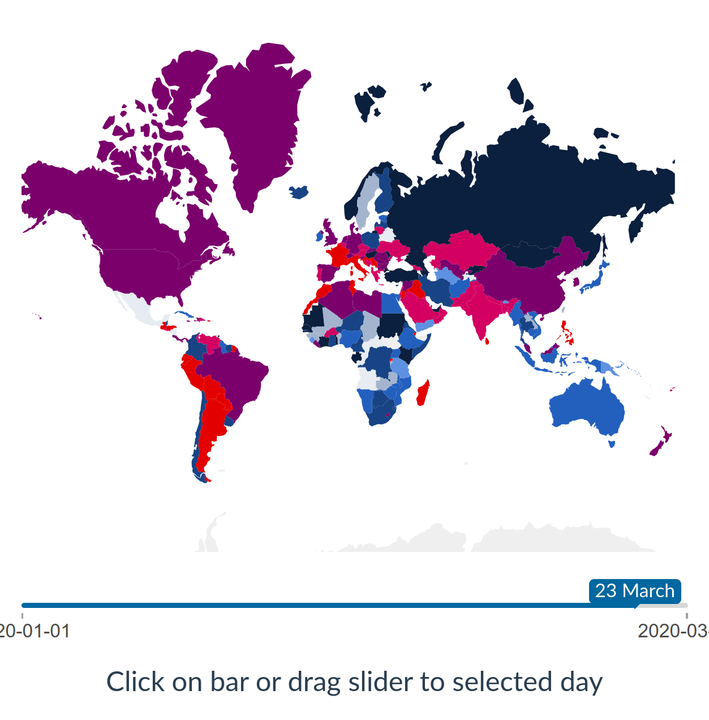
\includegraphics[width= 7cm]{Images/image_720.png}
\end{figure}
\begin{figure}[ht]
\centering
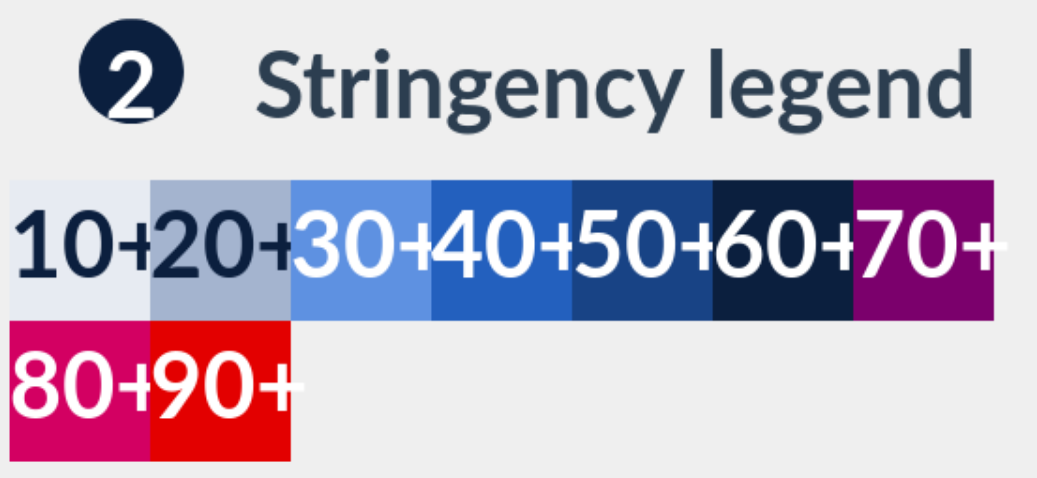
\includegraphics[width= 7cm]{Images/image.png}
\end{figure}

    \begin{tcolorbox}[breakable, size=fbox, boxrule=1pt, pad at break*=1mm,colback=cellbackground, colframe=cellborder]
\prompt{In}{incolor}{79}{\boxspacing}
\begin{Verbatim}[commandchars=\\\{\}]
\PY{c+c1}{\PYZsh{} fix different name of Czech Republic}
\PY{n}{dat}\PY{p}{[}\PY{l+s+s1}{\PYZsq{}}\PY{l+s+s1}{location}\PY{l+s+s1}{\PYZsq{}}\PY{p}{]}\PY{o}{.}\PY{n}{replace}\PY{p}{(}\PY{p}{\PYZob{}}\PY{l+s+s1}{\PYZsq{}}\PY{l+s+s1}{Czech Republic}\PY{l+s+s1}{\PYZsq{}}\PY{p}{:} \PY{l+s+s1}{\PYZsq{}}\PY{l+s+s1}{Czechia}\PY{l+s+s1}{\PYZsq{}}\PY{p}{\PYZcb{}}\PY{p}{,} \PY{n}{inplace} \PY{o}{=} \PY{k+kc}{True}\PY{p}{)}
\PY{n}{dat} \PY{o}{=} \PY{n}{dat}\PY{o}{.}\PY{n}{pivot}\PY{p}{(}\PY{n}{index}\PY{o}{=}\PY{l+s+s1}{\PYZsq{}}\PY{l+s+s1}{date}\PY{l+s+s1}{\PYZsq{}}\PY{p}{,}\PY{n}{columns}\PY{o}{=}\PY{l+s+s1}{\PYZsq{}}\PY{l+s+s1}{location}\PY{l+s+s1}{\PYZsq{}}\PY{p}{,}
                \PY{n}{values} \PY{o}{=} \PY{l+s+s1}{\PYZsq{}}\PY{l+s+s1}{stringency\PYZus{}index}\PY{l+s+s1}{\PYZsq{}}\PY{p}{)}
\PY{n}{dat}\PY{o}{.}\PY{n}{columns}\PY{o}{.}\PY{n}{name} \PY{o}{=} \PY{k+kc}{None}
\PY{n}{dat}\PY{o}{.}\PY{n}{reset\PYZus{}index}\PY{p}{(}\PY{n}{inplace}\PY{o}{=} \PY{k+kc}{True}\PY{p}{)}
\PY{n}{dat} \PY{o}{=} \PY{n}{dat}\PY{p}{[}\PY{n}{nations}\PY{p}{]}\PY{p}{[}\PY{l+m+mi}{1}\PY{p}{:}\PY{l+m+mi}{190}\PY{p}{]} \PY{c+c1}{\PYZsh{} Get rows from 01/01/2020 \PYZhy{} 08/07/2020}
\PY{c+c1}{\PYZsh{} Fill NaN by mean}
\PY{n}{mean\PYZus{}values} \PY{o}{=} \PY{n}{dat}\PY{o}{.}\PY{n}{mean}\PY{p}{(}\PY{n}{axis}\PY{o}{=}\PY{l+m+mi}{1}\PY{p}{)}
\PY{k}{for} \PY{n}{i}\PY{p}{,} \PY{n}{\PYZus{}} \PY{o+ow}{in} \PY{n+nb}{enumerate}\PY{p}{(}\PY{n}{dat}\PY{p}{)}\PY{p}{:}
    \PY{n}{dat}\PY{o}{.}\PY{n}{iloc}\PY{p}{[}\PY{p}{:}\PY{p}{,} \PY{n}{i}\PY{p}{]} \PY{o}{=} \PY{n}{dat}\PY{o}{.}\PY{n}{iloc}\PY{p}{[}\PY{p}{:}\PY{p}{,} \PY{n}{i}\PY{p}{]}\PY{o}{.}\PY{n}{fillna}\PY{p}{(}\PY{n}{mean\PYZus{}values}\PY{p}{)}
\PY{c+c1}{\PYZsh{} save data}
\PY{n}{file}\PY{o}{.}\PY{n}{save\PYZus{}pickle}\PY{p}{(}\PY{n}{dir\PYZus{}path}\PY{p}{[}\PY{l+s+s1}{\PYZsq{}}\PY{l+s+s1}{PROCESSED\PYZus{}DIR}\PY{l+s+s1}{\PYZsq{}}\PY{p}{]} \PY{o}{+} \PY{l+s+s1}{\PYZsq{}}\PY{l+s+s1}{/policy\PYZus{}stringency.pkl}\PY{l+s+s1}{\PYZsq{}}\PY{p}{,}
                 \PY{n}{dat}\PY{p}{)}
\PY{n}{dat}\PY{o}{.}\PY{n}{to\PYZus{}csv}\PY{p}{(}\PY{n}{dir\PYZus{}path}\PY{p}{[}\PY{l+s+s1}{\PYZsq{}}\PY{l+s+s1}{PROCESSED\PYZus{}DIR}\PY{l+s+s1}{\PYZsq{}}\PY{p}{]} \PY{o}{+} \PY{l+s+s1}{\PYZsq{}}\PY{l+s+s1}{/policy\PYZus{}stringency.csv}\PY{l+s+s1}{\PYZsq{}}\PY{p}{,}
           \PY{n}{index} \PY{o}{=} \PY{k+kc}{False}\PY{p}{)}
\end{Verbatim}
\end{tcolorbox}
    %%%%%%%%%%%%%%%%%%%%%%%%%%%%%%%
    \newpage
    \subsection{Exercise 4}
    \subsubsection{Background}
    At the moment, gorverment arount the world are implement many policies to stop the spreading of COVID-19.Therefore, we are really in the head of an effective way to measure the efficiency of our policy.\\
    However, due to the limited information about the current disease and the reliability of the data. It's hard to calculate and interpret the information.\\
    In this part, we are using the SIR model on the actual data, knowning the limitation of the our information and the over simplication of our assumpstions.\\
    In our case, we consider R is the number of people that could not get infected and could not spread the disease (recovered + death) \\
    We assume: \\
    The daily new recorded case $ X_1 = \frac{dR}{dt}$ $\sim$ Poission($\gamma I $)
    \begin{align} \label{x1}
        X_1 = \frac{dR}{dt} &\sim Poission(\gamma I ) = \gamma I_{t-1}
    \end{align}
    The daily new case $X_2$
    \begin{align} \label{x2}
        X_2 = \frac{dR}{dt} + \frac{dI}{dR} &= \frac{\beta}{N} I_{t-1} S_{t-1} = \beta I \sim Poission(\beta I)
    \end{align}
    In our data,
    \[
        \left\{
                \begin{array}{ll}
                  N \gg I \Rightarrow S \approx N-I-R\\
                  N \gg R
                \end{array}
              \right.
    \]
    We standardlized the two expressions \eqref{x1}, \eqref{x2} to Normal Distribution:
    \begin{align}
        Y_1 = \frac{X_1 - \gamma I}{\sqrt{\gamma I}} \sim N(0,1) \label{y1} \\
        Y_2 = \frac{X_2 - \beta I}{\sqrt{\beta I}} \sim N(0,1) \label{y2}
    \end{align}
    We want to know the development of he outbreak.If more and more people are affected:
    \begin{equation*}
        \frac{dI}{dt} > 0 \Leftrightarrow \frac{\beta}{N}IS - \gamma I > 0 \\
        \Leftrightarrow \beta I - \gamma I > 0 \Leftrightarrow \frac{\beta}{\gamma} > 1
    \end{equation*}
    We are interested in $R_0$ = $\frac{\beta}{\gamma}$
    \begin{equation*}
    \begin{split}
        E(R_0) &= \int \pi (\beta, \gamma | X) R_0 (\beta,\gamma) d(\beta,\gamma) \\
         &\propto \int \pi (X | \beta ,\gamma) \pi (\beta, \gamma) R_0(\beta, \gamma) d(\beta , \gamma) \\
         &\approx \sum_{i=1}^m \pi (X | \beta_i ,\gamma_i) \frac{\beta_i}{\gamma_i}
    \end{split}
    \end{equation*}
    where $(\beta_i ,\gamma_i)$ is selected  from the probability $\pi (\beta,\gamma)$ and $m$ is the size of sample. \\
    We consider  $\beta_i$ and $\gamma_i$  is independent
    \begin{equation}
        p(X|\beta_i ,\gamma_i) = p(Y_1|\beta_i ) p(Y_2|\gamma_i )
    \end{equation}
    As we've said before, $p(Y_1|\beta_i)$ and $p(Y_2|\gamma_i)$ are both follow the standard normal distribution N(0, 1), therefore:\\
    $$log(p(Y_1|\beta_i)) = \sum_{k=1}^n log(\frac{1}{\sqrt{2\pi}} e^{\frac{-Y^2_{1k}}{2}})$$
    $$log(p(Y_2|\gamma_i)) = \sum_{k=1}^n log(\frac{1}{\sqrt{2\pi}} e^{\frac{-Y^2_{2k}}{2}})$$
    where n is the lenght of our real data.\\
    It's here that we run into a computational problem: \\
    the result of this $p(Y_1|\beta_i)$ and $p(Y_2|\gamma_i)$ is extremely small, which make sense since technically, the probability of the random variable exactly equal any data point $P(Z = Y_{k}) = \int_{Y_{k}}^{Y_{k}} \frac{1}{\sqrt{2\pi}} e^{\frac{-Y^2_{1k}}{2}}$ for a continous distribution is, theoratically, zero.\\
    Even if we ignore the integral part and just calculate as $P(Z = Y_{k}) = \frac{1}{\sqrt{2\pi}} e^{\frac{-Y^2_{1k}}{2}}$, the result will be in the range of (0, 0.24) with maximum probability when $Y_k = 0$ (the mean of N(0, 1)). And that is just the probability of a SINGLE data point. We still have to multiply the probability of hundred of data points together. A single out of place data point with probability like 0.00000001 (which actually happen pretty frequently consider that real data is not perfectly fit the SIR model) will lower the whole result to nearly zero. It means that the more data we use, the lower our probability will become.\\
    Using the sum of log equation above, we can actually calculate how small that is: $log(p(Y_1|\beta_i))$ and $log(p(Y_2|\gamma_i))$ are both return result ranging -1000000000 to -1000, for any country data and with any combination of $\beta$ and $\gamma$.\\
    Our goal is to calculate the sum:
    $$\sum_{i=1}^m p(X | \beta_i ,\gamma_i) \frac{\beta_i}{\gamma_i}$$
    But since as explain above: $p(X | \beta_i ,\gamma_i)$ = at least $e^{-1000}$, any calculator we known of refuse to compute this to anything other than zero. making EVERY TERM of the sum become zero.
    \\ \\
    Due to the limitation and unreliability natural of our data, as well as to get at least a usable probability. We'll instead use a method of counting the ratio of number of data points that is inside an predetermined range over the data size:
    \begin{enumerate}
        \item Calculate the likelihood of $p(Y_1|\beta_i)$ and $p(Y_2|\gamma_i)$ with $Y_1 = {y_{11},y_{12},...,y_{1k}}$ and $Y_2 = {y_{21},y_{22},...,y_{2k}}$
        \item for j = 1 to k do:
        \subitem If $-1 < Y_{1j} < 1 $ $\Rightarrow$ We assume $p(Y_{1j}|\beta_i) = 1$ else $p(Y_{1j}|\beta_i) = 0$
        \subitem If $-1 < Y_{2j} < 1 $ $\Rightarrow$ We assume $p(Y_{2j}|\gamma_i) = 1$ else $p(Y_{2j}|\gamma_i) = 0$
        \item $p(Y_1|\beta_i)$ = $\frac{\sum p(Y_{1i}|\beta_i)}{k}$ 
        \item $p(Y_2|\gamma_i)$ = $\frac{\sum p(Y_{2i}|\gamma_i)}{k}$ 
    \end{enumerate}
    Note: the acceptance range from -1 to 1 is chosen arbitrary, for N(0, 1) this range will consist of about 69\% of the whole distribution density.
    
    \subsubsection{Analyzing The Basic Reproduction Number}
    By using the Metropolis–Hastings sampler in Exercise 3 and the COVID-19 data crawl from above, we can say that the policy and social distancing mostly effect the $R_0$ of each country, or say in another way that most of social distacing and policy help to control to the outbreak of COVID-19 for like: Belgium, France, Ireland, Italy, Poland, Romania, Spain, based on the result, the $R_0$ are noticeably lower than it should be.The $R_0$ of Denmark and Austria are higher than other country, that might be caused by the relatively lower rate of recovery of the country.
    \\
    Note: The $R_0$ values show below are not nesscessary equal to real worl $R_0$, those number should only proportional to $R_0$ by a constant.
    
\begin{center}
\begin{tabular}{ |c|c|c| } 
 \hline\hline
 Country & $R_0$ before policy and social distacing & $R_0$ after policy and social distacing \\ \hline\hline
 Austria & 0.30279562635924867     & 0.47733182616357916 \\ 
 Belgium & 3.7665788011525643     & 0.01373385814390452 \\
 Bulgaria & 0.4967450737872335     & 0.025249591452450305 \\ 
 Czechia & 0.44038749841738095     & 0.03558545686845637 \\
 Denmark & 0.658298474672732     & 4.4793434610138645 \\ 
 Finland & 8.989803159710142     & 1.6565768219909778 \\
 France & 5.082577434307611     & 0.02127603860161918 \\ 
 Germany & 1.4220286196555145   & 0.1413085381796394 \\
 Ireland & 2.13481804260756      & 0.6214845108555257 \\
 Italy & 18.986383356646446     & 0.03517023351281024 \\ 
 Poland & 1.3614887393274009     & 0.04391800148869624 \\
 Portugal & 0.3166099470870522     & 0.0025753927691526497 \\ 
 Romania & 20.303495188256115     & 0.6945603309617605\\
 Spain & 9.875606385089855     & 0.013824224373535546 \\ 
 \hline
\end{tabular}
\end{center}
    \begin{figure}[ht]
        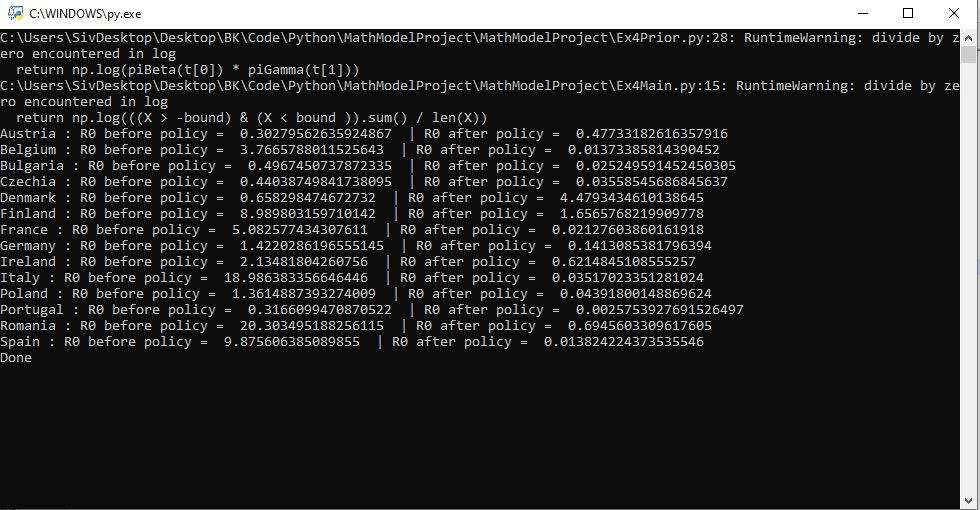
\includegraphics[width=\linewidth, center]{Images/ex4plot.png}
    \end{figure}
    
    \subsubsection{Implementation}
    Implementing exercise 4
    \\
    Calling MH sample for beta and gamma in Ex4Prior.py, which is the same as Ex3\_PriorSampling call but without the plotting part:
    \lstinputlisting[language=Python, firstline=1, lastline=26]{Implementations/Ex4Main.py}
    Loading real data crawed from github into the program:
    \lstinputlisting[language=Python, firstline=27, lastline=87]{Implementations/Ex4Main.py}
    Setting up the period before and after social distancing, then do the sum 
    $$\sum_{i=1}^m \pi (X | \beta_i ,\gamma_i) \frac{\beta_i}{\gamma_i} $$
    \lstinputlisting[language=Python, firstline=89, lastline=158]{Implementations/Ex4Main.py}
    
    %%%%%%%%%%%%%%%%%%%%%%%%%%%%%%%
    \subsection{Exercise 5}
    \subsubsection{Background}
    % Some Background Here
    
    % Inputs to compute using the machine learning
    
    % Outputs : Expected value of I and R
    
    % Explain Loss's Function (MSE)
    \textbf{Mean Squared Errors }\label{MSE} 
    \\
    \\
    \indent In machine learning, our main goal is to minimize the error which is defined by the Loss Function. And every type of Algorithm has different ways of measuring the error.
    \\
    \\
    \indent In statistics, the mean squared error (MSE) or mean squared deviation (MSD) of an estimator (of a procedure for estimating an unobserved quantity) measures the average of the squares of the errors—that is, the average squared difference between the estimated values and the actual value. 
    \\
    \\
    \indent The MSE assesses the quality of a predictor (i.e., a function mapping arbitrary inputs to a sample of values of some random variable), or an estimator (i.e., a mathematical function mapping a sample of data to an estimate of a parameter of the population from which the data is sampled). The definition of an MSE differs according to whether one is describing a predictor or an estimator. 
    \\
    \\
    \indent If a vector of n predictions is generated from a sample of n data points on all variables, and Y is the vector of observed values of the variable being predicted, with \^{Y} being the predicted values (e.g. as from a least-squares fit), then the within-sample MSE of the predictor is computed as. 
    \begin{equation*}
        \textcolor{blue}{MSE = \frac{1}{n} \sum_{i=1}^n (Y_i - \hat{Y_i})^2}
    \end{equation*}
    
    \textcolor{blue}{\textbf{Minimize Loss}( training process )}
    The most popular minimizer use some variation of \textcolor{blue}{gradient descent} which required the gradient of the loss function to be known. We want to obtain the optimal ($\beta$, $\gamma$) by performing first-order iterative optimization algorithm.
    \\
    
    \textbf{However}, this is very hard to achieve because the derivatives: $\frac{\delta I}{\delta \beta}$ and $\frac{\delta R}{\delta \gamma}$ is almost impossible to calculate.
    \\
    
    \textbf{Therefore}, we will not choose new $\beta$ and $\gamma$ based on any directions and instead random a new $\beta$ and $\gamma$ based on the current $\beta$ and $\gamma$ ( the ones produce the smallest loss ). To prevent falling indefinitly into local minima of the loss function, we will expanded the randomness(ie. standard deviation) for choosing new beta and gamma after a period amount of time has passed without finding smaller loss.
    \\
    
    \textbf{Moreover}, we need one more variable, which is the number of generation $m$, to stop the model or else it will go forever( because we never know which is the global minimum ).
    
    
    % Implementaion
    \subsubsection{Implementation}
     % Explain trainingLoss Function
    Our training loss function takes in:
    \begin{itemize}
        \item $\textbf{lossFunction}$: The function to calculate the loss value of the given data and the predicted data (produce using RK4's Algorithm with the initial beta and gamma).
        
        \item $\textbf{proposal}$: The function to produce new beta and gamma from the current beta and gamma followed normal distribution $N0$.
        
        \item $\textbf{data}$: represent the real data given by the .csv file.
        
        \item $\textbf{t0}$: an array of initial beta and gamma respectively.
        
        \item $\textbf{randomness}$: the initial randomness to be passed to the proposal which is used to find the closest $local minima$ of the loss.
        
        \item $\textbf{randomnessScaleFactor}$: scaling to increase used to bump up randomness at searching for a long time.
        
        \item $\textbf{searchTimeBeforeScaling}$: number of loop without found the new local minima off loss. This number will grow as the search area grows.
        
        \item $\textbf{m}$: number of accepted new \{ $\beta$, $\gamma$ \} that give the new local minimum loss.
    \end{itemize}
    $\textbf{Output}$:
    The ouput of our training function is the current loss and the most suitable \{ $\beta$, $\gamma$ \} founded.
        
    \lstinputlisting[language=Python, firstline = 6, lastline = 68]{Implementations/Ex5.py}
    
    % SIRlossFunction
    \textbf{\textcolor{blue}{SIRlossFunction}}: used to calculate the approximate loss of the predicted model and the real data.
    
    \lstinputlisting[language=Python, firstline = 70, lastline = 74]{Implementations/Ex5.py}
    
    % MSE Explaination
    \textbf{\textcolor{blue}{meanSquareError}}: calculate the approximate squared loss of the predicted data and the real data by the following formula:
    \\
    \textcolor{blue}{MSE = } $\frac{\sum(data - prediction)^2}{number of data}$
    \lstinputlisting[language=Python, firstline = 76, lastline = 77]{Implementations/Ex5.py}
    
    % Proposal Explaination
    \textbf{\textcolor{blue}{normalProposal}}: use to find new $\beta$ and $\gamma$ given in the random range
    \lstinputlisting[language=Python, firstline = 79, lastline = 89]{Implementations/Ex5.py}
   
   % take in the data from .csv
   \textbf{\textcolor{blue}{Retrieve data from .csv files}}
   \lstinputlisting[language=Python, firstline = 92, lastline = 138]{Implementations/Ex5.py}
   
   % Take in input and process loss function
   \textbf{\textcolor{blue}{Call user's inputs and log out the data in the console.}}
   \lstinputlisting[language=Python, firstline = 143, lastline = 167]{Implementations/Ex5.py}
   
   % Plot graph
   \textbf{\textcolor{blue}{Plot the graph for visualization}}
   \lstinputlisting[language=Python, firstline = 170, lastline = 200]{Implementations/Ex5.py}
   
    %%%%%%%%%%%%%%%%%%%%%%%%%%%%%%% 
    \subsubsection{Exercise 5 - Plotting Results}

    \begin{figure}[ht]
    \centering
    
    % Austria
    \textbf{\textcolor{blue}{Austria}}: 
    \begin{itemize}
        \item \textcolor{blue}{Start date}: 3/21/2020
        \item \textcolor{blue}{End date}: 7/7/2020
        \item Number of \textcolor{blue}{Generation}: \textcolor{blue}{10000}
        \item Final $\beta$: \textcolor{blue}{0.08261414389469697}
        \item Final $\gamma$: \textcolor{blue}{0.10616970863299684}
        \item \textcolor{blue}{Loss}: \textcolor{blue}{2900914.241658367}
    \end{itemize}
    
    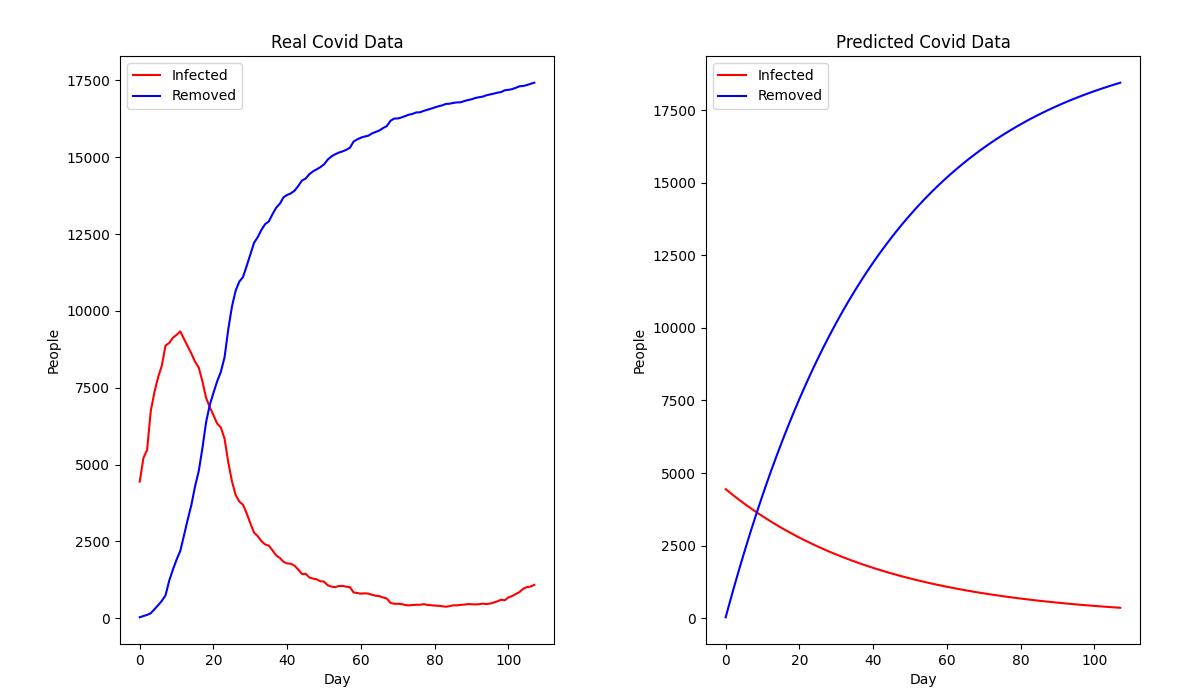
\includegraphics[width= \linewidth]{ex5-plot/Austria.png}
    
    \end{figure}
    
    \begin{figure}[ht]
    \centering
     % Belgium
    \textbf{\textcolor{blue}{Belgium}}: 
    \begin{itemize}
        \item \textcolor{blue}{Start date}: 3/21/2020
        \item \textcolor{blue}{End date}: 7/7/2020
        \item Number of \textcolor{blue}{Generation}: \textcolor{blue}{10000}
        \item Final $\beta$: \textcolor{blue}{0.04950314791362771}
        \item Final $\gamma$: \textcolor{blue}{0.023850517722867056}
        \item \textcolor{blue}{Loss}: \textcolor{blue}{145353181.81186876}
    \end{itemize}
    
    
    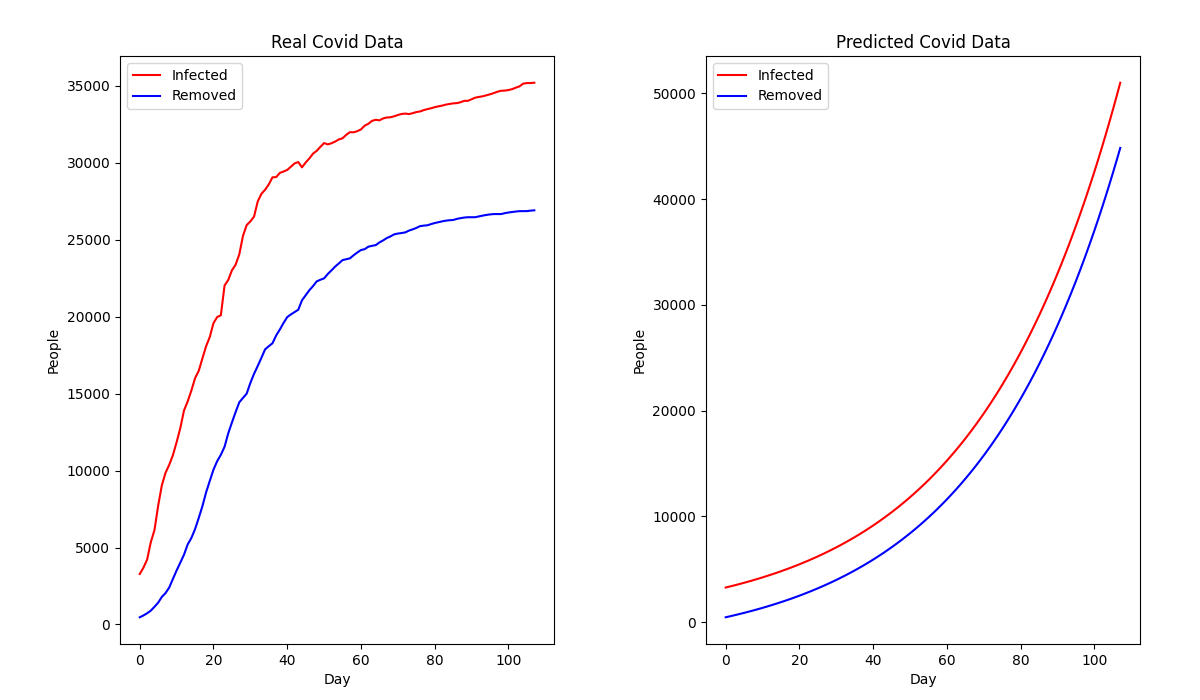
\includegraphics[width= \linewidth]{ex5-plot/Belgium.png}
    
    \caption{Belgium}
    \end{figure}
    
    \begin{figure}[ht]
    \centering
    % Czechia
    \textbf{\textcolor{blue}{Czechia}}: 
    \begin{itemize}
        \item \textcolor{blue}{Start date}: 3/21/2020
        \item \textcolor{blue}{End date}: 7/7/2020
        \item Number of \textcolor{blue}{Generation}: \textcolor{blue}{10000}
        \item Final $\beta$: \textcolor{blue}{0.055822538072428936}
        \item Final $\gamma$: \textcolor{blue}{0.04568700712825702}
        \item \textcolor{blue}{Loss}: \textcolor{blue}{2339607.771273511}
    \end{itemize}
    
    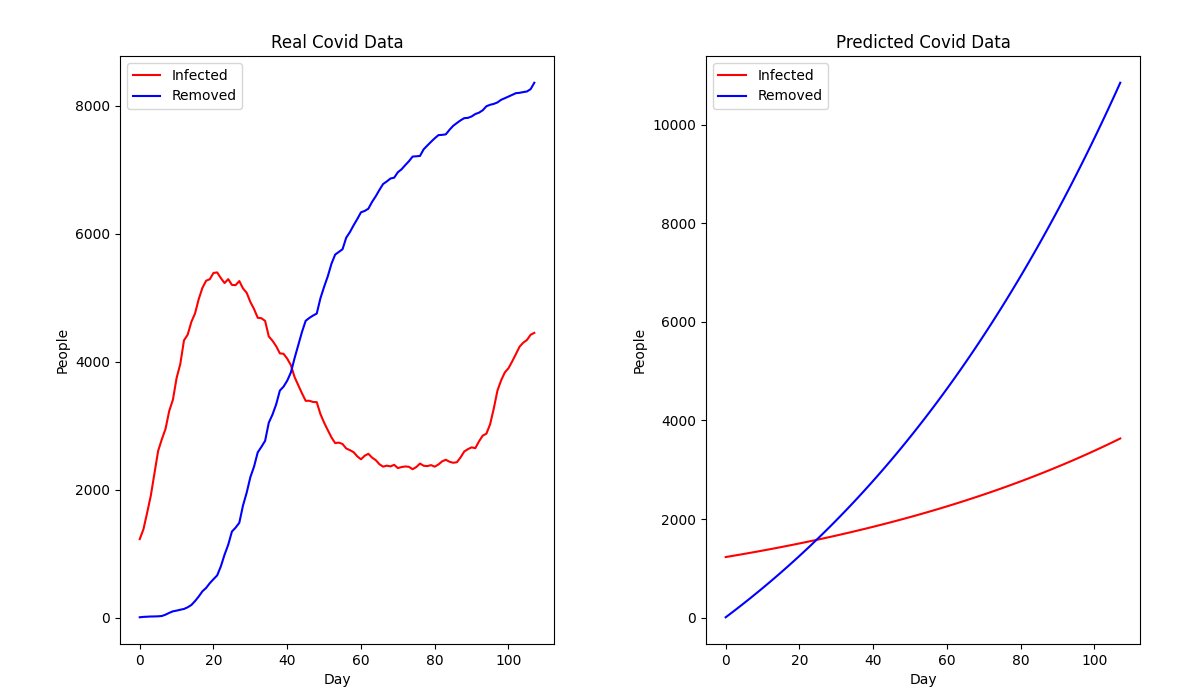
\includegraphics[width= \linewidth]{ex5-plot/Czechia.png}
    
    \caption{Czechia}
    \end{figure}
    \begin{figure}[ht]
    \centering
    % Denmark
    \textbf{\textcolor{blue}{Denmark}}: 
    \begin{itemize}
        \item \textcolor{blue}{Start date}: 3/21/2020
        \item \textcolor{blue}{End date}: 7/7/2020
        \item Number of \textcolor{blue}{Generation}: \textcolor{blue}{10000}
        \item Final $\beta$: \textcolor{blue}{0.1339769450044817}
        \item Final $\gamma$: \textcolor{blue}{0.14361893176363139}
        \item \textcolor{blue}{Loss}: \textcolor{blue}{850400.5881574824}
    \end{itemize}
    
    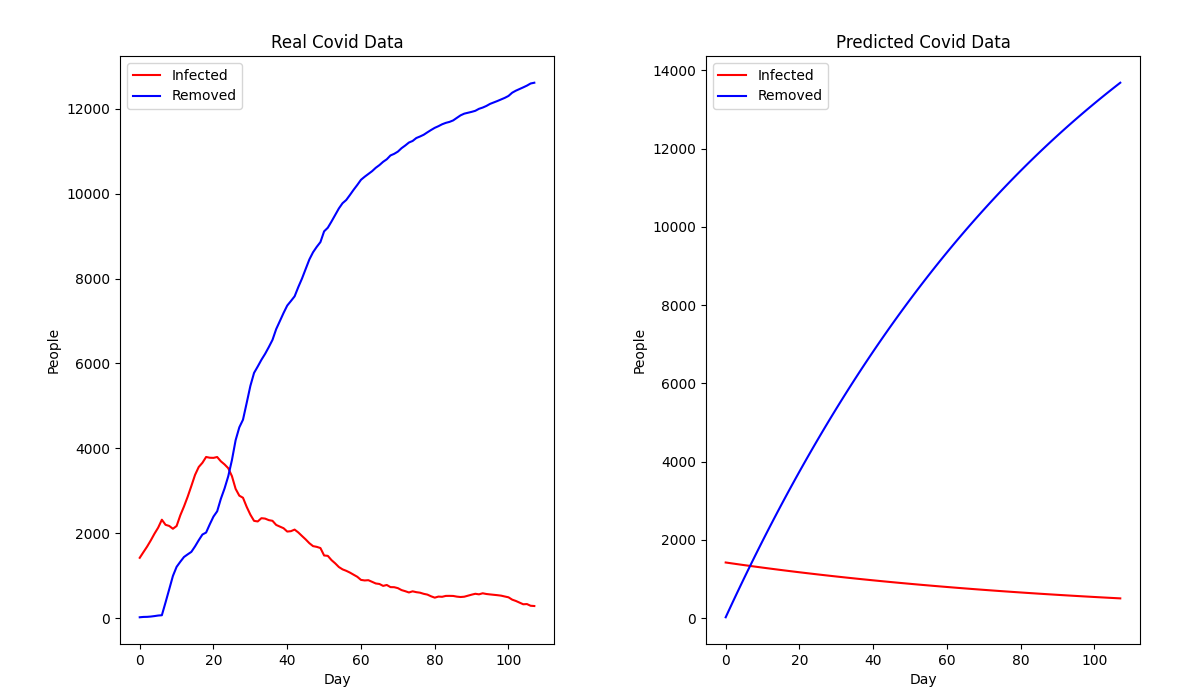
\includegraphics[width= \linewidth]{ex5-plot/Denmark.png}
    
    \caption{Denmark}
    \end{figure}
    
    \begin{figure}[ht]
    \centering
    % Finland
    \textbf{\textcolor{blue}{Finland}}: 
    \begin{itemize}
        \item \textcolor{blue}{Start date}: 3/21/2020
        \item \textcolor{blue}{End date}: 7/7/2020
        \item Number of \textcolor{blue}{Generation}: \textcolor{blue}{10000}
        \item Final $\beta$: \textcolor{blue}{0.114039185029659}
        \item Final $\gamma$: \textcolor{blue}{0.11487348612529852}
        \item \textcolor{blue}{Loss}: \textcolor{blue}{493898.796715808}
    \end{itemize}
    
    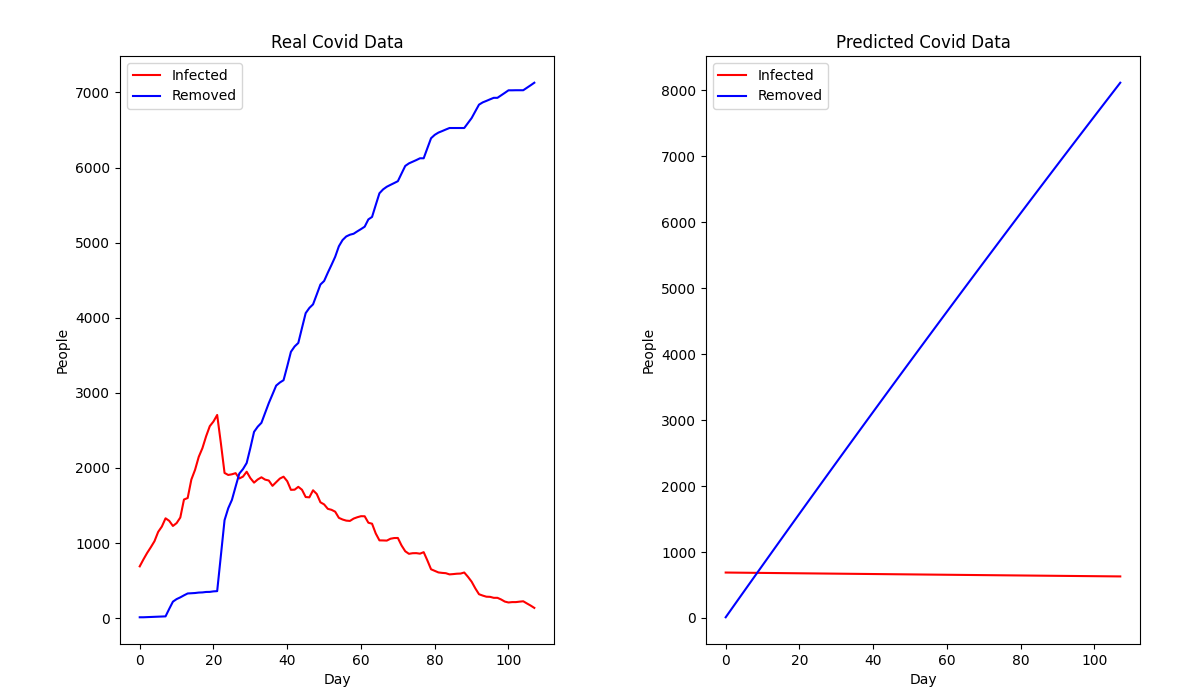
\includegraphics[width= \linewidth]{ex5-plot/Finland.png}
    
    \caption{Finland}
    \end{figure}
    
    \begin{figure}[ht]
    \centering
    % France
    \textbf{\textcolor{blue}{France}}: 
    \begin{itemize}
        \item \textcolor{blue}{Start date}: 3/21/2020
        \item \textcolor{blue}{End date}: 7/7/2020
        \item Number of \textcolor{blue}{Generation}: \textcolor{blue}{10000}
        \item Final $\beta$: \textcolor{blue}{0.04633654638644967}
        \item Final $\gamma$: \textcolor{blue}{0.027170784222120638}
        \item \textcolor{blue}{Loss}: \textcolor{blue}{1239411674.187388}
    \end{itemize}
    
    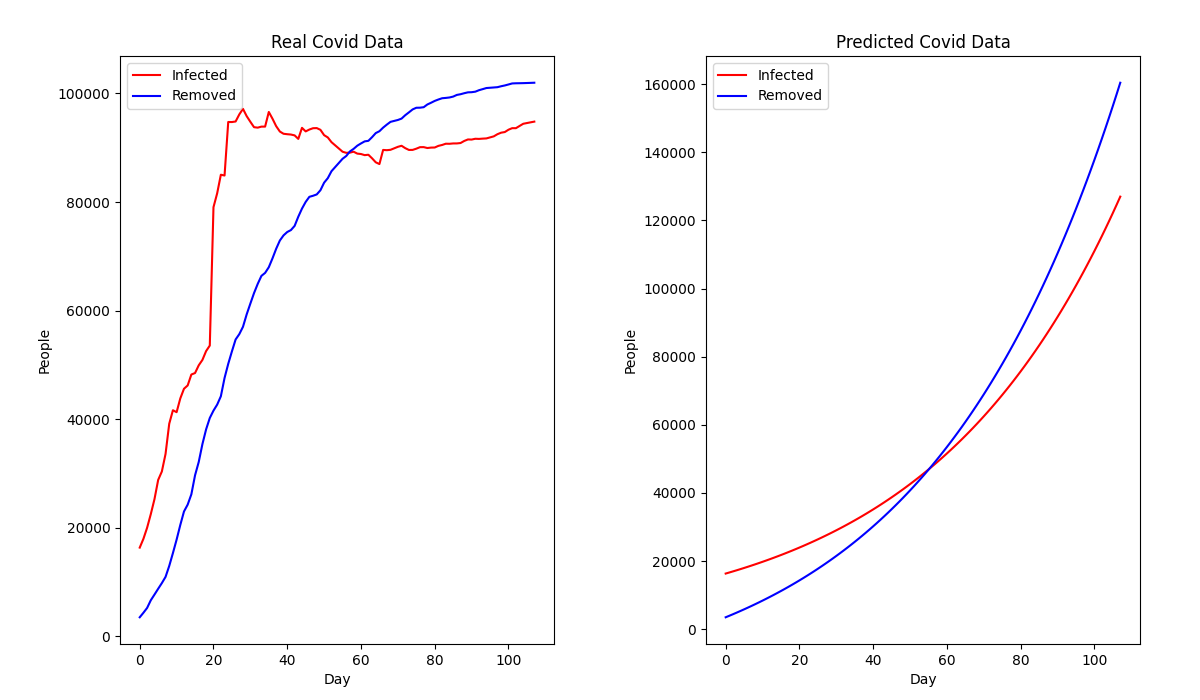
\includegraphics[width= \linewidth]{ex5-plot/France.png}
    
    \caption{France}
    \end{figure}
    \begin{figure}[ht]
    \centering
    % Germany
    \textbf{\textcolor{blue}{Germany}}: 
    \begin{itemize}
        \item \textcolor{blue}{Start date}: 3/21/2020
        \item \textcolor{blue}{End date}: 7/7/2020
        \item Number of \textcolor{blue}{Generation}: \textcolor{blue}{10000}
        \item Final $\beta$: \textcolor{blue}{0.1362806160946653}
        \item Final $\gamma$: \textcolor{blue}{0.1529868333277667}
        \item \textcolor{blue}{Loss}: \textcolor{blue}{277737758.93634045}
    \end{itemize}
    
    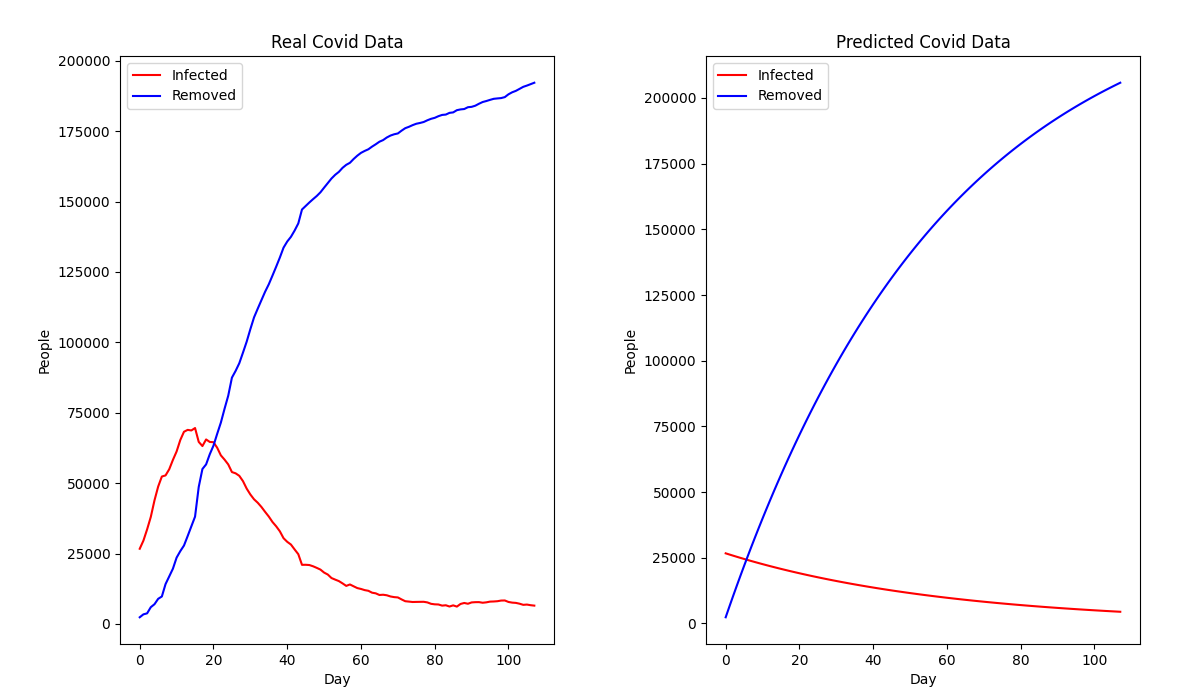
\includegraphics[width= \linewidth]{ex5-plot/Germany.png}
    
    \caption{Germany}
    \end{figure}
    %%%%%%%%%%%%%%%%%%%%%%%%%%%%%%%%%%%%%%%%%
    %Viet 
    \begin{figure}[ht]
    \centering
    \textbf{\textcolor{blue}{Ireland}}: 
    \begin{itemize}
        \item \textcolor{blue}{Start date}: 3/21/2020
        \item \textcolor{blue}{End date}: 7/7/2020
        \item Number of \textcolor{blue}{Generation}: 10000
        \item Final $\beta$: \textcolor{blue}{0.3259669200892496}
        \item Final $\gamma$: \textcolor{blue}{0.3318723646336088}
        \item \textcolor{blue}{Loss}: \textcolor{blue}{15315810.569687268}
    \end{itemize}
    
    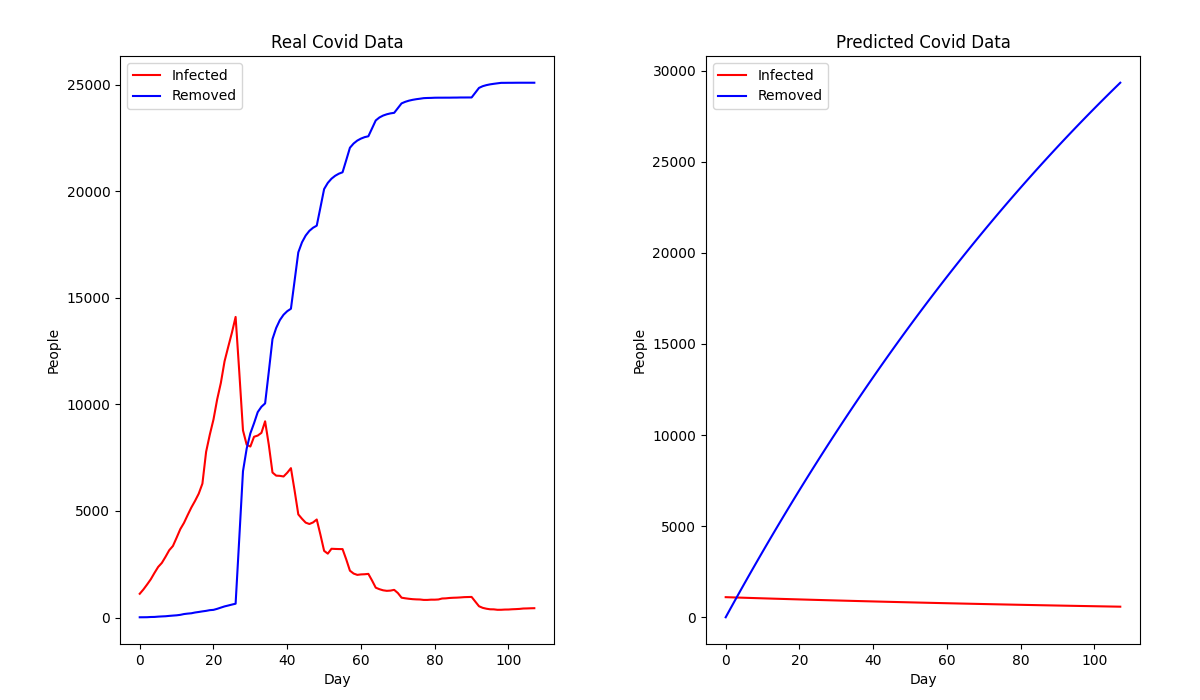
\includegraphics[width= \linewidth]{ex5-plot/Ireland.png}
    \caption{Ireland}
     \end{figure} 
     
     \begin{figure}[ht]
    \centering
    \textbf{\textcolor{blue}{Italy}}: 
    \begin{itemize}
        \item \textcolor{blue}{Start date}: 3/21/2020
        \item \textcolor{blue}{End date}: 7/7/2020
        \item Number of \textcolor{blue}{Generation}: 10000
        \item Final $\beta$: \textcolor{blue}{0.04747182556627497}
        \item Final $\gamma$: \textcolor{blue}{0.0491518304164244}
        \item \textcolor{blue}{Loss}: \textcolor{blue}{676299376.2818551}
    \end{itemize}
    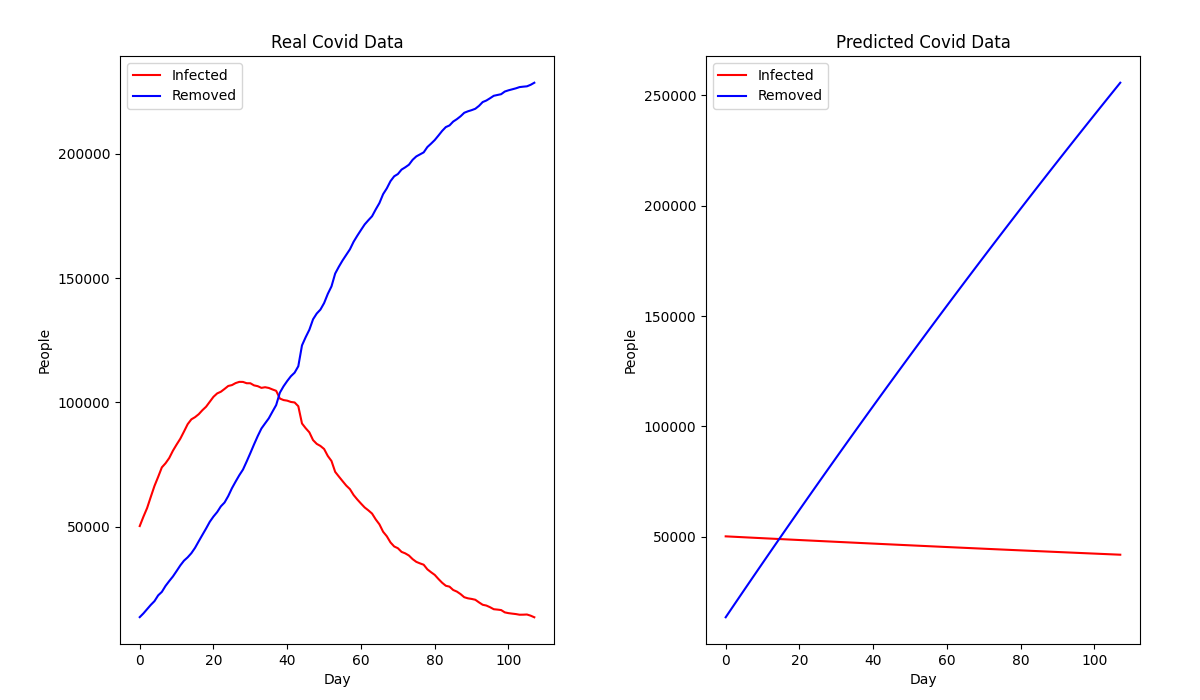
\includegraphics[width= \linewidth]{ex5-plot/Italy.png}
    \caption{Italy}
     \end{figure}
     
     \begin{figure}[ht]
    \centering
    \textbf{\textcolor{blue}{Poland}}: 
    \begin{itemize}
        \item \textcolor{blue}{Start date}: 3/21/2020
        \item \textcolor{blue}{End date}: 7/7/2020
        \item Number of \textcolor{blue}{Generation}: 10000
        \item Final $\beta$: \textcolor{blue}{0.08280057631634499}
        \item Final $\gamma$: \textcolor{blue}{0.05261566866900815}
        \item \textcolor{blue}{Loss}: \textcolor{blue}{15200404.856771646}
    \end{itemize}
    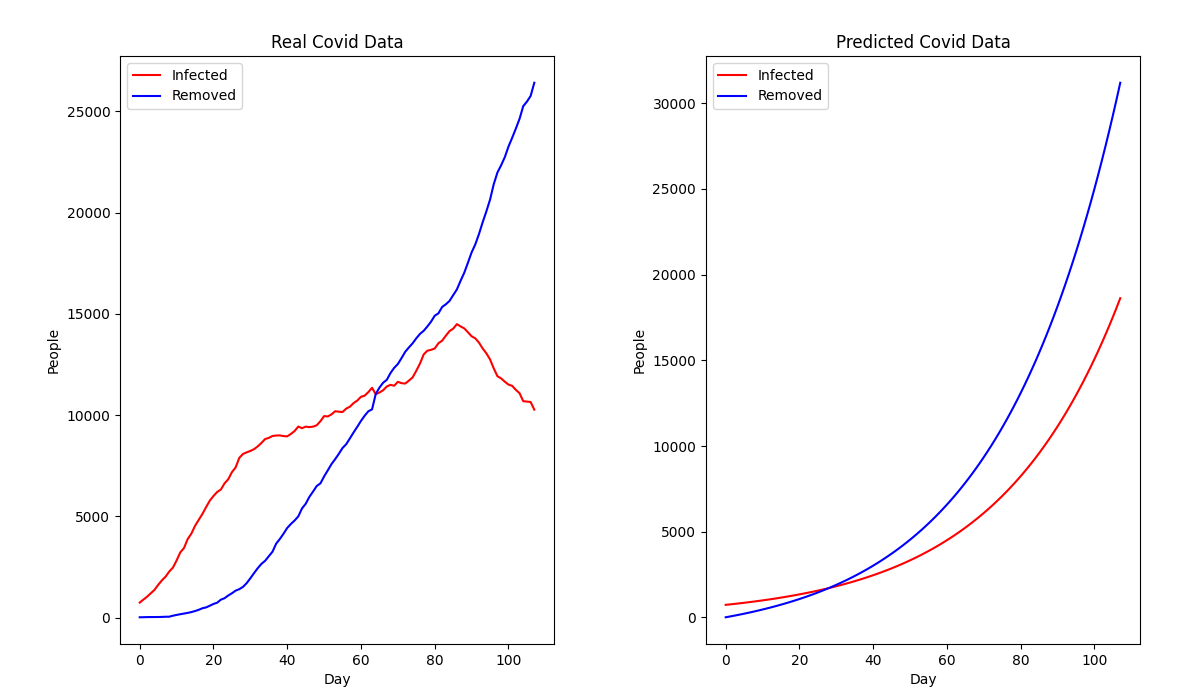
\includegraphics[width= \linewidth]{ex5-plot/Poland.png}
    \caption{Poland}
     \end{figure}
     
    \begin{figure}[ht]
    \centering
    \textbf{\textcolor{blue}{Portugal}}: 
    \begin{itemize}
        \item \textcolor{blue}{Start date}: 3/21/2020
        \item \textcolor{blue}{End date}: 7/7/2020
        \item Number of \textcolor{blue}{Generation}: 10000
        \item Final $\beta$: \textcolor{blue}{0.06566296591854241}
        \item Final $\gamma$: \textcolor{blue}{0.043766732501216765}
        \item \textcolor{blue}{Loss}: \textcolor{blue}{64874679.73756245}
    \end{itemize}
    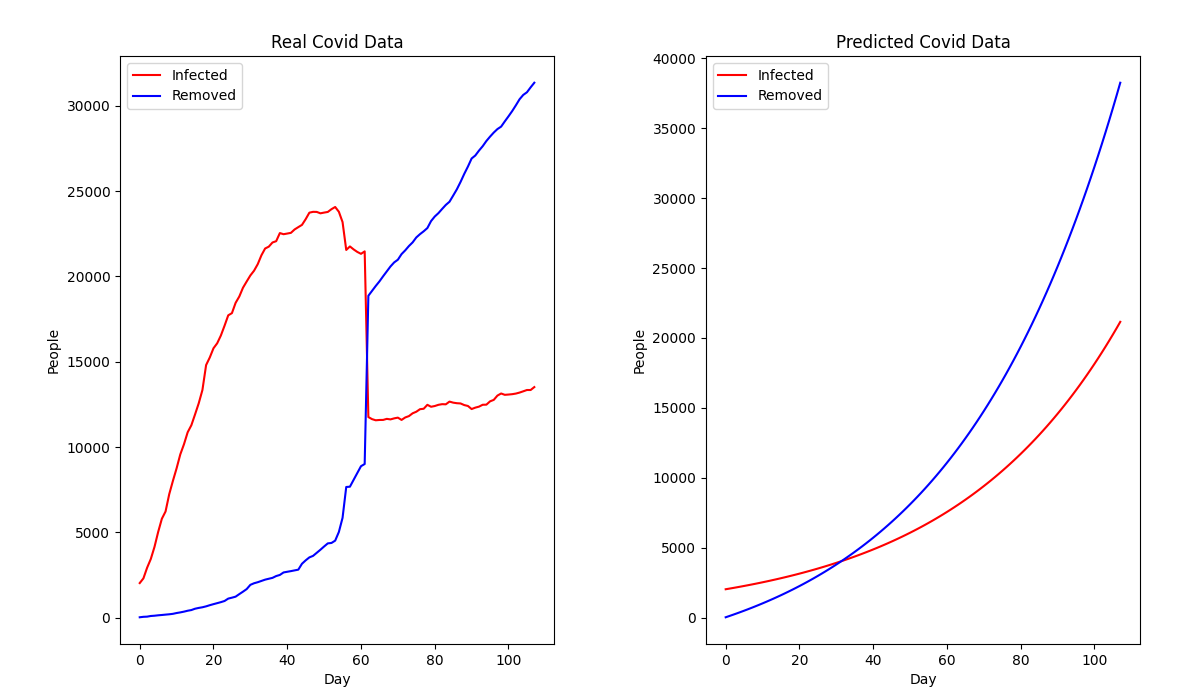
\includegraphics[width= \linewidth]{ex5-plot/Portugal.png}
    \caption{Portugal}
     \end{figure}
     
    \begin{figure}[ht]
    \centering
    \textbf{\textcolor{blue}{Romania}}: 
    \begin{itemize}
        \item \textcolor{blue}{Start date}: 4/20/2020
        \item \textcolor{blue}{End date}: 6/14/2020
        \item Number of \textcolor{blue}{Generation}: 10000
        \item Final $\beta$: \textcolor{blue}{0.04155789340282452}
        \item Final $\gamma$: \textcolor{blue}{0.04781414893777089}
        \item \textcolor{blue}{Loss}: \textcolor{blue}{363462.5800399513}
    \end{itemize}
    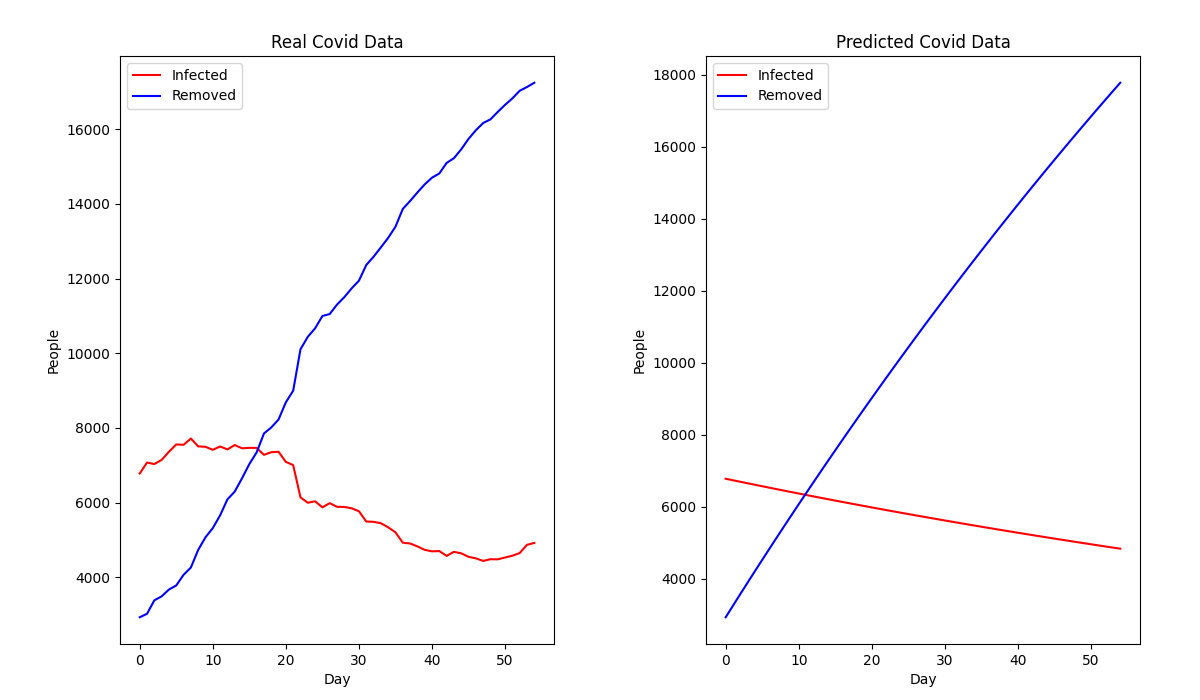
\includegraphics[width= \linewidth]{ex5-plot/Romania.png}
    \caption{Romania}
     \end{figure}
    \begin{figure}[ht]
    \centering
    \textbf{\textcolor{blue}{Spain}}: 
    \begin{itemize}
        \item \textcolor{blue}{Start date}: 3/31/2020
        \item \textcolor{blue}{End date}: 5/20/2020
        \item Number of \textcolor{blue}{Generation}: 10000
        \item Final $\beta$: \textcolor{blue}{0.043141937893975184}
        \item Final $\gamma$: \textcolor{blue}{0.045273619630837356}
        \item \textcolor{blue}{Loss}: \textcolor{blue}{116182856.16206549}
    \end{itemize}
    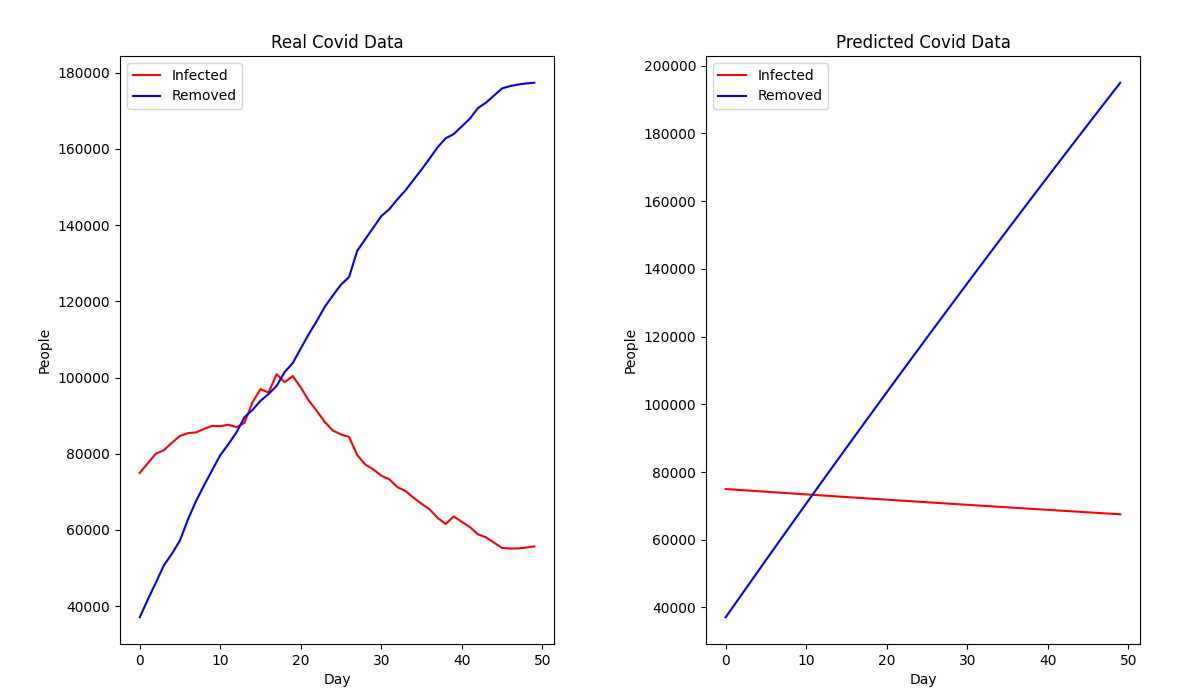
\includegraphics[width= \linewidth]{ex5-plot/Spain.png}
    \caption{Spain}
    \end{figure}
    
    \clearpage
    \section{Conclusion}
    As governments continue to respond to COVID-19, it is imperative to study what measures are effective and which are not. While the information presented here do, of course, can not describe and predict the whole situation, they can provide useful insights that help governments adopted an evidence-based approach to the measures they deploy.

It is our hope that scholars, medical professionals, policymakers, and concerned citizens will make use of our information to enhance all countries’ response. \\
\addcontentsline{toc}{section}{References}
\begin{thebibliography}{5}

\bibitem{a} S. T. Ho Lam and A. Suchard Marc. Simple MCMC under SIR. 2005. URL: \href{https://cran.r-project.org/web/packages/MultiBD/vignettes/SIR-MCMC.pdf}{https://cran.r-project.org/web/packages/MultiBD/vignettes/SIR-MCMC.pdf} 

\bibitem{b} T. Wu Joseph, Leung Kathy, and Leung Gabriel. “Nowcasting and forecasting the
potential domestic and international spread of the 2019-nCoV outbreak originating
in Wuhan, China: a modelling study”. In: 395 (2020).

\bibitem{c} Frank Giordano, William P Fox, and Steven Horton. A first course in mathematical
modeling. Nelson Education, 2013.

\bibitem{d} W. K. Hastings. “Monte Carlo Sampling Methods Using Markov Chains and Their
Applications”. In: Biometrika 57 (1) (1970), pp. 97–109.

\bibitem{e} Luca Magri and Nguyen Anh Khoa Doan. “First-principles Machine Learning for
COVID-19 Modeling”. In: arXiv preprint arXiv:2004.09478 (2020)
\end{thebibliography}


\end{document}